\subsection{滤子化集合上定义的实值函数}

命题 1. 设 \(f\) 与 \(g\) 是定义在集合 \(\mathbf{X}\) （它由滤子 \(\mathfrak{F}\) 滤子化）上的两个实值函数。若 \(\lim_{\mathfrak{F}} f\) 与 \(\lim_{\mathfrak{F}} g\) 存在，且对每个子集 \(\mathbf{A} \in \mathfrak{F}\) 存在 \(x \in \mathbf{A}\) 使得 \(f(x) \leqslant g(x)\) ，则我们有 \(\lim_{\mathfrak{F}} f \leqslant \lim_{\mathfrak{F}} g\) 。

为证明这一结果，我们将证明下述等价的命题：

命题 2. 设 \(f\) 与 \(g\) 是定义在集合 \(X\) （它由滤子 \(\mathfrak{F}\) 滤子化）上的两个实值函数。若 \(\lim_{\mathfrak{F}} f\) 与 \(\lim_{\mathfrak{F}} g\) 存在，且 \(\lim_{\mathfrak{F}} f > \lim_{\mathfrak{F}} g\) ，则存在一个集 \(A \in \mathfrak{F}\) ，使得 \(f(x) > g(x)\) 对一切 \(x \in A\) 成立。

设 \(a = \lim_{\mathfrak{F}} f\) ，设 \(b = \lim_{\mathfrak{F}} g\) ，并设 \(c\) 满足 \(b < c < a\) 。区间 \(]c, +\infty]\) （属于 \(\overline{\mathbf{R}}\) ）（相应地，\([-\infty, c[)\) ）是 \(a\) （相应地，\(b\) ）的邻域；因此存在一个集 \(M \in \mathfrak{F}\) （相应地，一个集 \(N \in \mathfrak{F}\) ），使得 \(f(x) > c\) 对一切 \(x \in M\) 成立{[}相应地，\(g(x) < c\) 对一切 \(x \in N\) 成立{]}。集 \(A = M \cap N\) 属于 \(\mathfrak{F}\) ，且 \(f(x) > c > g(x)\) 对一切 \(x \in A\) 成立。

作为命题 1 的一个特例，我们有下述定理：

定理 1（不等式延拓原理）. 设 \(f\) 与 \(g\) 是定义在集合 \(\mathbf{X}\) （它由滤子 \(\mathfrak{F}\) 滤子化）上的两个实值函数。若 \(\lim_{\mathfrak{F}} f\) 与 \(\lim_{\mathfrak{F}} g\) 存在，且 \(f \leqslant g\) ，则 \(\lim_{\mathfrak{F}} f \leqslant \lim_{\mathfrak{F}} g\) 。

\pandocbounded{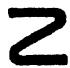
\includegraphics[keepaspectratio]{images/part002_67e89114.jpg}}

注. 特别地，若 \(f(x) < g(x)\) 对一切 \(x \in X\) 成立（或者只对滤子 \(\overline{\mathbf{R}}\) 的某一个集中的各点成立），则由定理 1 可以推出 \(\lim_{\mathfrak{F}} f \leqslant \lim_{\mathfrak{F}} g\) ；但我们不能推出严格不等式 \(\lim_{\mathfrak{F}} f < \lim_{\mathfrak{F}} g\) 。例如，取 \(X\) 为自然数集 \(N\) ，赋以 Fréchet 滤子，且设 \(f(n) = 0\) ，\(g(n) = 1/n\) ，则 \(f(n) < g(n)\) 对一切 \(n\) 成立，但 \(\lim_{n \to \infty} f(n) = \lim_{n \to \infty} f(n) = 0\) 。因此，在严格不等式中过渡到极限时，严格性会丢失。

定理 2（单调极限定理）. 设 X 是一个有序集，A 是 X 的一个有向子集 (*)。每个定义在 A 上的单调实值函数 f 关于 A 都有极限（第一章，§ 7，第 3 节）；若 f 递增（相应地，递减），则此极限等于集 \(f(A) \subset \overline{\mathbf{R}}\) 的上确界（相应地，下确界）。

例如设 \(f\) 递增，并令 \(a = \sup f(A)\) 。若 \(a = -\infty\) ，定理是平凡的。若 \(a > -\infty\) ，则对每个 \(b < a\) 存在 \(x \in A\) 使得 \(b < f(x) \leqslant a\) ；于是，若 \(S_x\) 是 \(A\) 的相对于 \(x\) 的截面（即所有 \(y \geqslant x\) 所成之集，参看第一章，§ 6，第 3 节），则 \(f(S_x)\) 含于 \(]b, +\infty]\) （它是 \(a\) 的一个邻域）之中，定理得证。若 \(f\) 递减，证明类似。

推论. 定义在有序集 X 的有向子集 A 上的递增（相应地，递减）实值函数，关于 A 有有限极限的充分必要条件是它在 A 中上有界（相应地，下有界）。

若把定理 2 应用于 \(\mathbf{A} = \mathbf{X} = \mathbf{N}\) （按关系 \(\leqslant\) 定序）的情形，就得到下述命题：

命题 3. 每个实数单调序列在 R 中有极限。特别地，由有限数组成的递增（相应地，递减）序列，当其上有界（相应地，下有界）时收敛于一个有限实数，否则收敛于 +∞（相应地，-∞）。例如，正整数序列收敛于 +∞。

这一事实正是用记号 \(\lim_{n\to \infty}u_n\) 表示序列极限的由来（第一章，§ 7，第 3 节）。

同样，每个严格递增的整数序列 \((p_n)\) 收敛于 \(+\infty\) ；因为由归纳法可见，\(p_n \geqslant p_0 + n\) 对一切 \(n\) 成立。

\subsection{实变量函数的右极限与左极限}

设 A 是 \(\overline{R}\) 的一个非空子集，且设 \(a \neq -\infty\) 是 \(\overline{R}\) 中位于集 \(B = A \cap [-\infty, a[\) 的闭包中的一点。集 B 关于关系 \(\leqslant\) 有向，它的截面滤子 F 与 a 在 \(\overline{R}\) 中的邻域滤子在 B 上的迹相同。

定义 2. 设 \(f\) 是定义在一个非空子集 \(A\) （属于 \(\overline{\mathbf{R}}\) ）上、取值于一个拓扑空间 \(X\) 中的函数。\(f\) 关于滤子 \(\mathfrak{F}\) 的极限（若存在）称为 \(f\) 在点 \(a\) 处关于 \(A\) 的左极限，记作

\(\lim_{x \to a, x < a, x \in \mathbf{A}} f(x), \text{ 或 } f(a - ), \text{ 若 } \mathbf{X} \text{ 是 Hausdorff 的。}\)

同样，若 \(a\) 位于集 \(A \cap ]a, +\infty]\) 的闭包中，我们定义 \(f\) 在点 \(a\) 处的右极限（若存在），并把它记作 \(\lim_{x \to a, x > a, x \in A} f(x)\) ，或 \(f(a+)\) ，如果 \(X\) 是豪斯多夫的。

下述命题是定理 2 的一个直接推论：

命题 4. 设 A 是 \(\overline{\mathbf{R}}\) 的一个子集，且设 \(a \neq -\infty\) 是交集 \(\mathbf{A} \cap [-\infty, a[\) 的闭包中的一点。若 \(f\) 是定义在 A 上的单调实值函数，则 \(f\) 有左极限 \(f(a - )\) （在 \(a\) 处且关于 A ）。

\subsection{实值函数的界}

定义 3. 设 \(f\) 是定义在集合 \(\mathbf{X}\) 上的实值函数，\(\mathbf{A}\) 是 \(\mathbf{X}\) 的一个非空子集。此时集 \(f(\mathbf{A})\) 在 \(\overline{\mathbf{R}}\) 中的上确界（相应地，下确界）称为 \(f\) 在 \(\mathbf{A}\) 中的上确界（相应地，下确界），记作 \(\sup_{x\in \mathbf{A}}f(x)\left[\text{resp. } \inf_{x\in \mathbf{A}} f(x)\right]\) 。

特别地，若 A 是 \(\overline{R}\) 的一个非空子集，则

\[
\sup \mathrm{A} = \sup _ {x \in \mathrm{A}} x.\tag{1}
\]

用右端的记号来表示 A 的上确界，往往更为方便。

数 \(a = \sup_{x \in \mathbf{A}} f(x)\) 由下列两条性质刻画：

\begin{enumerate}
\def\labelenumi{(\roman{enumi})}
\item
  对一切 \(x \in \mathbf{A}, f(x) \leqslant a\) 。
\item
  对每个 \(b < a\) ，存在 \(x \in \mathbf{A}\) 使得 \(b < f(x) \leqslant a\) 。
\end{enumerate}

数 \(\sup_{x\in\mathbf{A}}f(x)\) 与 \(\inf_{x\in\mathbf{A}}f(x)\) 属于 \(f(\mathbf{A})\) 在 \(\overline{\mathbf{R}}\) 中的闭包。我们有 \(\inf_{x\in\mathbf{A}}f(x)\leqslant\sup_{x\in\mathbf{A}}f(x)\) ；且这两个数相等当且仅当 \(f\) 在 \(\mathbf{A}\) 上取常值。

定义在集合 X 上的实值函数在 X 的一个非空子集 A 中上有界（相应地，下有界）当且仅当 \(\sup_{x\in\mathbf{A}}f(x)<+\infty\) {[}相应地，\(\inf_{x\in\mathbf{A}}f(x)>-\infty\) {]}。f 在 A 中有界当且仅当 \(|f|\) 在 A 中上有界，亦即当且仅当 \(\sup_{x\in\mathbf{A}}|f(x)|<+\infty\) 。

我们有

\[
\inf _ {x \in \mathbf {A}} f (x) = - \sup _ {x \in \mathbf {A}} (- f (x)).\tag{2}
\]

这一关系式把下确界的所有性质都化归为上确界的性质；因此在一般情况下我们只谈论后者。

命题 5. 设 \(f\) 是定义在集合 \(\mathbf{X}\) 上的一个实值函数。在集 \(\mathfrak{F}(\mathbf{X})\) （由 \(\mathbf{X}\) 的所有有限子集组成，按关系 \(\subset\) 有向）上，实值函数 \(\mathbf{H} \to \sup_{x \in \mathbf{H}} f(x)\) 是递增的，实值函数 \(\mathbf{H} \to \inf_{x \in \mathbf{H}} f(x)\) 是递减的，并且我们有

\[
\left\{ \begin{array}{l} \sup _ {x \in \mathbf {A}} f (x) = \lim _ {\mathbf {H} \in \mathfrak {F} (\mathbf {X})} (\sup _ {x \in \mathbf {H}} f (x)), \\ \inf _ {x \in \mathbf {A}} f (x) = \lim _ {\mathbf {H} \in \mathfrak {F} (\mathbf {X})} (\inf _ {x \in \mathbf {H}} f (x)). \end{array} \right.\tag{3}
\]

设 \(\varphi(\mathbf{H}) = \sup_{x \in \mathbf{H}} f(x)\) 。显然 \(\varphi\) 递增，因而有极限 \(a\) （第 2 节，定理 2）；又因对一切 H 有 \(\varphi(\mathbf{H}) \leqslant \sup_{x \in \mathbf{A}} f(x)\) ，故有 \(a \leqslant \sup_{x \in \mathbf{A}} f(x)\) （第 2 节，定理 1）。倘若 \(a < \sup_{x \in \mathbf{A}} f(x)\) ，就会存在 \(x_0 \in \mathbf{X}\) 使得 \(a < f(x_0)\) ；但这是矛盾的，因为 \(\varphi(\mathbf{H}) \geqslant f(x_0)\) （只要 \(x_0 \in \mathbf{H}\) ）。

特别地，由 (1)，若 A 是 \(\overline{R}\) 的任意一个非空子集，则我们有

\[
\sup \mathrm{A} = \lim _ {\mathrm{H} \in \mathfrak {F} (\mathrm{A})} (\sup _ {x \in \mathrm{H}} x).\tag{4}
\]

命题 6. 设 \(f\) 与 \(g\) 是定义在 \(\mathbf{X}\) 上的两个实值函数。若 \(f(x) \leqslant g(x)\) 对每一点 \(x\) （属于某个非空子集 \(A\) ，而该子集含于 \(\mathbf{X}\) ）成立，则我们有

\[
\left\{ \begin{array}{l} \sup _ {x \in \mathbf {A}} f (x) \leqslant \sup _ {x \in \mathbf {A}} g (x), \\ \inf _ {x \in \mathbf {A}} f (x) \leqslant \inf _ {x \in \mathbf {A}} g (x). \end{array} \right.\tag{5}
\]

命题 7. 设 \(f\) 是定义在 \(\mathbf{X}\) 上的一个实值函数。若 \(\mathbf{A}\) 与 \(\mathbf{B}\) 是 \(\mathbf{X}\) 的两个非空子集，且 \(\mathbf{A} \subset \mathbf{B}\) ，则

\[
\sup _ {x \in \mathbf {A}} f (x) \leqslant \sup _ {x \in \mathbf {B}} f (x).\tag{6}
\]

命题 8. 设 \(f\) 是定义在 \(\mathbf{X}\) 上的一个实值函数，且设 \((\mathbf{A}_t)_{t \in I}\) 是由 \(\mathbf{X}\) 的非空子集组成的一个非空族；则

\[
\sup_{x\in \bigcup_{t\in \mathbf{I}}\mathbf{A}_{t}}f(x) = \sup_{t\in \mathbf{I}}(\sup_{x\in \mathbf{A}_{t}}f(x)).\tag{7}
\]

设 \(f\) 是定义在乘积集合 \(\mathbf{X}_1 \times \mathbf{X}_2\) 上的一个实值函数。若 \(\mathbf{A}_2\) 是 \(\mathbf{X}_2\) 的一个非空子集，我们用 \(\sup_{x_2 \in \mathbf{A}_2} f(x_1, x_2)\) 表示在 \(\mathbf{A}_2\) 中取的上确界，即实值函数 \(x_2 \to f(x_1, x_2)\) （定义在 \(\mathbf{X}_2\) 上）的上确界。由命题 8 我们特别推出：

命题 9. 设 \(f\) 是定义在乘积集合 \(\mathbf{X}_1 \times \mathbf{X}_2\) 上的一个实值函数。若 \(\mathbf{A}_1, \mathbf{A}_2\) 分别是 \(\mathbf{X}_1, \mathbf{X}_2\) 的任意非空子集，则

\[
\sup _ {(x _ {1}, x _ {2}) \in \mathbf {A} _ {1} \times \mathbf {A} _ {2}} f (x _ {1}, x _ {2}) = \sup _ {x _ {1} \in \mathbf {A} _ {1}} (\sup _ {x _ {2} \in \mathbf {A} _ {2}} f (x _ {1}, x _ {2})) = \sup _ {x _ {2} \in \mathbf {A} _ {2}} (\sup _ {x _ {1} \in \mathbf {A} _ {1}} f (x _ {1}, x _ {2})).\tag{8}
\]

\subsection{实值函数族的包络}

定义 4. 设 \((f_{t})_{t\in I}\) 是定义在集合 X 上的一个实值函数族。在每一点 \(x\in X\) 处取值为 \(\sup_{t\in I}(f_t(x))\) {[}相应地，inf \((f_t(x))]\) 的 X 上的实值函数称为族 \((f_t)\) 的上包络（相应地，下包络），记作 \(\sup_{t\in I}f_{t}\) 或 \(\sup_{t}f_{t}\) （相应地，inf \(f_{t}\) 或 inf \(f_{t}\) ）。

族 \((f_{t})\) 的上包络就是这个族在定义于 X 上的实值函数的格 \(\overline{R}\) 中的上确界，这也就说明了记号 \(\sup f_{t}\) 的合理性。

此外，若给 \(\overline{\mathbf{R}}^{\mathbf{X}}\) 赋以其诸因子的拓扑（都与 \(\overline{R}\) 的拓扑相同）的乘积所成的拓扑，则我们有下述命题：

命题 10. 在积空间 \(\overline{\mathbf{R}}^{\mathbf{X}}\) 中，上包络 \(\sup f_{t}\) （实值函数族 \((f_{t})_{t\in I}\) 的上包络）是关于有向集 \(\mathfrak{F}(\mathbf{I})\) （由 \(\mathbf{I}\) 的有限子集组成）对映射 \(\mathrm{H}\to \sup_{t\in \mathbf{H}}f_t\) 取的极限{[}该映射把每个有限子集 \(\mathrm{H}\) （属于 \(\mathbf{I}\) ）映到有限子族 \((f_{t})_{t\in H}]\) 的上包络。

这由第 4 节的命题 5 以及第一章，§ 7，第 6 节，命题 10 的推论 1 立即得出。

因此我们可以写

\[
\sup _ {t \in I} f _ {t} = \lim _ {H \in \mathfrak {F} (I)} \left(\sup _ {t \in H} f _ {t}\right).\tag{9}
\]

定义 5. 实值函数族 \((f_t)_{i\in I}\) （定义在集合 \(\mathbf{X}\) 上）称为在 \(\mathbf{X}\) 中一致上有界（相应地，一致下有界）的，如果存在一个有限数 \(a\) ，使得 \(f_{t}(x) \leqslant a\) {[}相应地，\(f_{t}(x) \geqslant a\) {]} 对一切 \(x \in X\) 和一切 \(t \in I\) 成立。族 \((f_{t})\) 称为在 \(X\) 中一致有界的，如果它在 \(X\) 中既一致上有界又一致下有界。

于是，\((f_{t})\) 在 \(\mathbf{X}\) 中一致上有界当且仅当该族的上包络在 \(\mathbf{X}\) 中上有界。\((f_{t})\) 在 \(\mathbf{X}\) 中一致有界当且仅当族 \((|f_{t}|)\) 的上包络在 \(\mathbf{X}\) 中上有界{[}亦即当且仅当存在一个有限实数 \(a \geqslant 0\) ，使得 \(|f_{t}(x)| \leqslant a\) 对一切 \(x \in \mathbf{X}\) 和一切 \(t \in I\) 都成立 {]}。

\subsection{实值函数关于滤子的上极限与下极限}

设 \(f\) 是定义在集合 \(\mathbf{X}\) （它由滤子 \(\mathfrak{G}\) 滤子化）上的实值函数。\(\mathfrak{G}\) 关于关系 \(\supset\) 是一个有向集（第一章，§ 6）。对每个 \(\mathbf{M} \in \mathfrak{G}\) 考虑实数 \(\sup_{x \in \mathbf{M}} f(x)\) ：这样便得到函数 \(\mathbf{M} \to \sup_{x \in \mathbf{M}} f(x)\) （它定义在 \(\mathfrak{G}\) 上而取值于 \(\overline{\mathbf{R}}\) ），根据第 4 节命题 7，它是 \(\mathfrak{G}\) 上的递减函数。于是由第 2 节定理 2，它关于有向集 \(\mathfrak{G}\) 有极限。

定义 6. 实值函数 \(\mathbf{M} \to \sup_{x \in \mathbf{M}} f(x)\) 关于有向集 \(\mathfrak{G}\) 的极限称为 \(f\) 关于滤子 \(\mathfrak{G}\) 的上极限，记作 \(\lim \sup_{\mathfrak{G}} f\) ，或 \(\lim \sup_{x, \mathfrak{G}} f(x)\) 。

\(f\) 关于滤子 \(\mathfrak{G}\) 的下极限类似地定义，并记作 \(\liminf_{\mathfrak{G}} f\) 或 \(\liminf_{x, \mathfrak{G}} f(x)\) 。于是我们有

\[
\left\{ \begin{array}{l} \lim \sup_{\mathfrak{G}} f = \lim_{\mathbf {M} \in \mathfrak {G}}(\sup_{x \in \mathbf {M}}f(x)), \\ \lim \inf_{\mathfrak{G}} f = \lim_{\mathbf {M} \in \mathfrak {G}}(\inf_{x \in \mathbf {M}}f(x)). \end{array} \right.\tag{10}
\]

通常在记号中略去滤子 \(\mathfrak{G}\) ，而简单地写 \(\lim \sup f\) 或 \(\lim \sup_x f(x)\) ，或在不会引起混淆时写 \(\lim \sup f(x)\) 。

由公式 (10) 与定理 1，我们得到

\[
\inf _ {x \in \mathbf {X}} f (x) \leqslant \lim \inf _ {\mathfrak {G}} f \leqslant \lim \sup _ {\mathfrak {G}} f \leqslant \sup _ {x \in \mathbf {X}} f (x).\tag{11}
\]

由第 2 节定理 2，我们也可以写

\[
\left\{\lim \sup _ {\mathfrak {G}} f = \inf _ {\mathbf {M} \in \mathfrak {G}} (\sup _ {x \in \mathbf {M}} f (x)), \right.\tag{12}
\]

\[
\left\{\lim \inf _ {\mathfrak {G}} f = \sup _ {\mathbf {M} \in \mathfrak {G}} (\inf _ {x \in \mathbf {M}} f (x)). \right.
\]

又，在公式 (10) 与 (12) 的右端，可以把滤子 \(\mathfrak{G}\) 换成任意一个基 \(\mathfrak{B}\) （\(\mathfrak{G}\) 的基）。

由 (2) 与 (10)，

\[
\lim \inf _ {\mathfrak {G}} f = - \lim \sup _ {\mathfrak {G}} (- f)\tag{13}
\]

因此我们只需考虑上极限。

定理 3. 实值函数 \(f\) 关于滤子 \(\mathfrak{G}\) 的上极限等于 \(f\) 关于 \(\mathfrak{G}\) 的最大聚值。

设 \(b\) 是 \(f\) 关于 \(\mathfrak{G}\) 的一个聚点。对每个 \(\mathbf{M} \in \mathfrak{G}\) ，\(b\) 属于 \(f(\mathbf{M})\) 的闭包，因此 \(b \leqslant \sup_{x \in \mathbf{M}} f(x)\) ，从而由 (12) 得 \(b \leqslant \limsup_{\mathfrak{G}} f = a\) 。

另一方面，设 V 是 a 在 \(\overline{R}\) 中的任意一个开邻域。那么存在 G 中的一个集合 \(M_{0}\) ，使得对每个 \(M \in G\) （它含于 \(M_{0}\) ），都有 \(\sup_{x \in M} f(x) \in V\) ；由于 V 是开集，\(f(M)\) 与 V 相交，因此 a 是 f 关于 G 的一个聚点，证毕。

推论 1. 为使 \(\limsup_{\mathfrak{G}}f = \liminf_{\mathfrak{G}}f\) ，必须且只需 \(f\) 关于滤子 \(\mathfrak{G}\) 有极限，且此时

\[
\lim _ {\mathfrak {G}} f = \lim \sup _ {\mathfrak {G}} f = \lim \inf _ {\mathfrak {G}} f.
\]

因为 \(\overline{\mathbf{R}}\) 是紧的，滤子基 \(f(\mathfrak{G})\) 有极限点当且仅当它只有一个聚点（第一章，§ 9，第 1 节，定理 1 的推论）。

推论 2. 若 \(\mathfrak{H}\) 是比 \(\mathfrak{G}\) 更细的滤子，则我们有

\[
\lim \inf _ {\mathfrak {G}} f \leqslant \lim \inf _ {\mathfrak {H}} f \leqslant \lim \sup _ {\mathfrak {H}} f \leqslant \lim \sup _ {\mathfrak {G}} f.
\]

因为 \(f\) 关于 \(\mathfrak{H}\) 的每个聚点也是 \(f\) 关于 \(\mathfrak{G}\) 的聚点（第一章，§ 7，第 3 节）。

特别地，若 \(\lim_{\mathfrak{H}}f\) 存在，则

\[
\lim \inf _ {\mathfrak {G}} f \leqslant \lim _ {\mathfrak {H}} f \leqslant \lim \sup _ {\mathfrak {G}} f.
\]

推论 3. 设 A 是滤子 G 中的一个集合，\(\mathfrak{G}_{\mathbf{A}}\) 是 G 在 A 上诱导的滤子，\(f_{\mathbf{A}}\) 是 \(f\) 在 A 上的限制，则

\[
\lim \sup _ {\mathfrak {G} _ {\mathbf {A}}} f _ {\mathbf {A}} = \lim \sup _ {\mathfrak {G}} f.
\]

因为滤子基 \(f(\mathfrak{G})\) 的每个聚点也是滤子基 \(f_{\mathrm{A}}(\mathfrak{G}_{\mathrm{A}})\) 的聚点，反之亦然。

由于这个原因，若 \(f\) 只定义在一个子集 \(A\) （含于 \(X\) 且属于 \(\mathfrak{G}\) ）上，则常滥用记号写 \(\limsup_{\mathfrak{G}} f\) 以代替 \(\limsup_{\mathfrak{G}_{\mathbf{A}}} f_{\mathbf{A}}\) 。

命题 11. 设 \(f\) 与 \(g\) 是定义在滤子化集合 \(X\) 上的两个实值函数。则关系 \(f \leqslant g\) 蕴含

\[
\left\{ \begin{array}{l} \lim \sup f \leqslant \lim \sup g, \\ \lim \inf f \leqslant \lim \inf g. \end{array} \right.\tag{14}
\]

这是关系式 (12) 的直接推论。

当 X 是拓扑空间且 \(\mathfrak{G}\) 是 X 的一点 \(a\) 的邻域滤子时，我们写 \(\limsup_{x\to a}f(x)\) {[}相应地，\(\liminf_{x\to a}f(x)]\) 以代替 \(\limsup_{\mathfrak{G}}f\) {[}相应地，\(\liminf_{\mathfrak{G}}f]\) ；显然我们有

\[
\liminf _ {x \to a} f (x) \leqslant f (a) \leqslant \limsup _ {x \to a} f (x).\tag{15}
\]

更一般地，若 X 是拓扑空间 Y 的子空间，且 G 是一点 \(a \in \overline{X}\) 的邻域滤子在 X 上的迹，我们写 \(\limsup_{x \to a, x \in X} f(x)\) {[}相应地，\(\liminf_{x \to a, x \in X} f(x)\) {]}以代替 \(\limsup_{\mathfrak{G}} f\) {[}相应地，\(\liminf_{\mathfrak{G}} f\) {]}；\(\limsup_{x \to a, x \in X} f(x)\) 称为当 x 趋于 a 且保持在 X 中时 \(f(x)\) 的上极限。若 X 是 \(\{a\}\) 的余集，则在这些记号中我们用`` \(x \neq a\) ''代替`` \(x \in X\) ''。

若 \(\mathbf{A}\) 是 \(\mathbf{X}\) 的一个子集且 \(a \in \overline{\mathbf{A}}\) ，则（定理 3 的推论 2）

\[
\liminf _ {x \to a, x \in \mathbf {X}} f (x) \leqslant \liminf _ {x \to a, x \in \mathbf {A}} f (x) \leqslant \limsup _ {x \to a, x \in \mathbf {A}} f (x) \leqslant \limsup _ {x \to a, x \in \mathbf {X}} f (x).
\]

若 V 是 \(a\) 在 Y 中的一个邻域，则有（定理 3 的推论 3）

\[
\lim \sup _ {x \to a, x \in \mathbf {V} \cap \mathbf {X}} f (x) = \lim \sup _ {x \to a, x \in \mathbf {X}} f (x).
\]

因此，拓扑空间中一点处的上极限与下极限概念，和极限概念一样，具有局部特征。

最后，若 \(\mathfrak{G}\) 是 \(\mathbf{N}\) 上的 Fréchet 滤子，则关于 \(\mathfrak{G}\) ，映射 \(n \to u_n\) （它把 \(\mathbf{N}\) 映入 \(\overline{\mathbf{R}}\) ）的上极限（相应地，下极限）记作 \(\limsup_{n \to \infty} u_n\) （相应地，\(\liminf_{n \to \infty} u_n\) ），并称为实数序列 \(u_n\) 的上极限（相应地，下极限）。

于是，关系式 \(\limsup_{n\to \infty}u_n = a\in \mathbb{R}\) 等价于下述论断：对任意给定的 \(\varepsilon >0\) ，存在整数 \(n_0\) ，使得对每个 \(n\geqslant n_0\) 有 \(u_{n}\leqslant a + \varepsilon\) ，且对无穷多个 \(n\) 的值有 \(u_{n}\geqslant a - \varepsilon\) 。当序列上极限的值为 \(+\infty\) 或 \(-\infty\) 时，其定义可以类似地翻译过来。

给定实值函数的序列 \((f_n)\) （定义在集合 \(\mathbf{X}\) 上），我们用 \(\limsup_{n\to \infty}f_n\) （相应地，\(\liminf_{n\to \infty} f_n\) ）表示在任一点 \(x\in \mathbf{X}\) 处取值为 \(\limsup_{n\to \infty}f_n(x)\) {[}相应地，\(\liminf_{n\to \infty} f_n(x)\) {]}的实值函数。由 (10) 与 (12) 我们推出

\[
\left\{\begin{array}{l}\lim \sup _ {n \rightarrow \infty} f _ {n} = \inf _ {n \in \mathbb {N}} (\sup _ {m \geqslant n} f _ {m}) = \lim _ {n \rightarrow \infty} (\sup _ {m \geqslant n} f _ {m}),\\\lim \inf _ {n \rightarrow \infty} f _ {n} = \sup _ {n \in \mathbb {N}} (\inf _ {m \geqslant n} f _ {m}) = \lim _ {n \rightarrow \infty} (\inf _ {m \geqslant n} f _ {m}),\end{array}\right.\tag{16}
\]

其中的极限是在积空间 \(\overline{\mathbf{R}}^{\mathbf{X}}\) 中取的。序列 \((f_n)\) 在 \(\overline{\mathbf{R}}^{\mathbf{X}}\) 中有极限当且仅当 \(\limsup_{n\to\infty}f_n=\liminf_{n\to\infty}f_n\) （定理 3 的推论 1，以及第一章，§ 7，第 6 节，命题 10 的推论 1）。

\subsection{实值函数的代数运算}

设 \(f\) 与 \(g\) 是定义在集合 \(\mathbf{X}\) 上的两个实值函数；如果和 \(f(x) + g(x)\) {[}相应地，积 \(f(x)g(x)\) {]}对一切 \(x \in \mathbf{X}\) 有定义，则我们用 \(f + g\) （相应地，\(fg\) ）表示实值函数

\[
x \rightarrow f (x) + g (x) \quad [ \text { resp. } x \rightarrow f (x) g (x) ].
\]

同样，若 \(1 / f(x)\) 对一切 \(x\in \mathbf{X}\) 有定义，则 \(1 / f\) 表示函数 \(x\to 1 / f(x)\) 。

因此只要 \(f\) 不取值 \(0\) ，这最后一个函数便有定义；当 \(f\) 在区间 \([0, +\infty]\) （相应地，\([-\infty, 0]\) ）中取值时，\(1/f(x)\) 在约定 \(1/0 = +\infty\) （相应地，\(1/0 = -\infty\) ）之下便处处有定义；在这种情形函数 \(1/f\) 有定义。

设 X 由滤子 \(\mathfrak{F}\) 滤子化，且 \(\lim_{\mathfrak{F}} f\) 与 \(\lim_{\mathfrak{F}} g\) 存在。若一方面函数 \(f + g\) （相应地，\(fg\) ，\(1/g\) ）有定义，另一方面表达式 \(\lim_{\mathfrak{F}} f + \lim_{\mathfrak{F}} g\) （相应地，\(\lim_{\mathfrak{F}} f\) . \(\lim_{\mathfrak{F}} g\) ，\(1/\lim_{\mathfrak{F}} f\) ）有意义，则 \(\lim_{\mathfrak{F}} (f + g)\) {[}相应地，\(\lim_{\mathfrak{F}} fg\) ，\(\lim_{\mathfrak{F}} (1/f)\) {]}存在且等于该表达式，这是由于函数 \(x + y\) （相应地，\(xy\) ，\(1/x\) ）在其有定义的点处连续。

命题 12. 设 \(f\) 与 \(g\) 是定义在集合 \(\mathbf{X}\) 上的两个实值函数，并设 \(\mathbf{A}\) 是 \(\mathbf{X}\) 的一个非空子集。

\textit{(i) 我们有}

\begin{enumerate}
\def\labelenumi{(\arabic{enumi})}
\setcounter{enumi}{16}
\tightlist
\item
\end{enumerate}

\[
\sup _ {x \in \mathbf {A}} (f (x) + g (x)) \leqslant \sup _ {x \in \mathbf {A}} f (x) + \sup _ {x \in \mathbf {A}} g (x),\tag{17}
\]

\[
\sup _ {x \in \mathbf {A}} f (x) + \inf _ {x \in \mathbf {A}} g (x) \leqslant \sup _ {x \in \mathbf {A}} (f (x) + g (x)),\tag{18}
\]

只要这些不等式两边都有定义。

\begin{enumerate}
\def\labelenumi{(\roman{enumi})}
\setcounter{enumi}{1}
\tightlist
\item
  若 \(f(x)\) 与 \(g(x)\) 都 \(\geqslant 0\) （对每个 \(x \in \mathbf{A}\) ），则
\end{enumerate}

\begin{enumerate}
\def\labelenumi{(\arabic{enumi})}
\setcounter{enumi}{18}
\tightlist
\item
\end{enumerate}

\[
\sup _ {x \in \mathbf {A}} (f (x) g (x)) \leqslant \sup _ {x \in \mathbf {A}} f (x) \sup _ {x \in \mathbf {A}} g (x),\tag{19}
\]

\[
\sup _ {x \in \mathbf {A}} f (x) \inf _ {x \in \mathbf {A}} g (x) \leqslant \sup _ {x \in \mathbf {A}} (f (x) g (x))\tag{20}
\]

只要这些不等式两边都有定义。

\begin{enumerate}
\def\labelenumi{(\roman{enumi})}
\setcounter{enumi}{2}
\tightlist
\item
  若 \(f(x) \geqslant 0\) （对一切 \(x \in \mathbf{A}\) ），则
\end{enumerate}

\[
\sup _ {x \in \mathbf {A}} (1 / f (x)) = \inf _ {x \in \mathbf {A}} f (x)\tag{21}
\]

（约定 \(1 / 0 = +\infty\) ）。

设 \(\mathbf{H}\) 是 \(\mathbf{A}\) 的任意一个有限子集。若 \(x_0\) 是 \(\mathbf{H}\) 中使 \(f + g\) 取其最大值的点之一，则我们有

\[
f (x _ {0}) + g (x _ {0}) \leqslant \sup _ {x \in \mathbf {H}} f (x) + \sup _ {x \in \mathbf {H}} g (x);
\]

另一方面，若 \(x_{1}\) 是 \(H\) 中使 \(f\) 取其最大值的点之一，则

\[
f (x _ {1}) + g (x _ {1}) \geqslant \sup _ {x \in \mathbf {H}} f (x) + \inf _ {x \in \mathbf {H}} g (x);
\]

因此

\[
\sup _ {x \in \mathbf {H}} f (x) + \inf _ {x \in \mathbf {H}} g (x) \leqslant \sup _ {x \in \mathbf {H}} (f (x) + g (x)) \leqslant \sup _ {x \in \mathbf {H}} f (x) + \sup _ {x \in \mathbf {H}} g (x).
\]

把第 4 节命题 5 与第 2 节定理 1 应用于此，即得不等式 (17) 与 (18)。其余不等式的证明是类似的。

推论 1. 设 \(f\) 是定义在 \(\mathbf{X}\) 上的实值函数，\(k\) 是实数。则

\[
\sup _ {x \in \mathbf {A}} (f (x) + k) = k + \sup _ {x \in \mathbf {A}} f (x)\tag{22}
\]

只要两边都有定义；又若 \(k \geqslant 0\) ，则

\[
\sup _ {x \in \mathbf {A}} (k f (x)) = k. \sup _ {x \in \mathbf {A}} f (x)\tag{23}
\]

只要两边都有定义。

推论 2. 设 \(f_{1}\) 与 \(f_{2}\) 是分别定义在集合 \(X_{1}, X_{2}\) 上的两个实值函数；则若 \(A_{1}, A_{2}\) 分别是 \(X_{1}, X_{2}\) 的任意非空子集，我们有

\[
\sup _ {(x _ {1}, x _ {2}) \in \mathbf {A} _ {1} \times \mathbf {A} _ {2}} (f _ {1} (x _ {1}) + f _ {2} (x _ {2})) = \sup _ {x _ {1} \in \mathbf {A} _ {1}} f _ {1} (x _ {1}) + \sup _ {x _ {2} \in \mathbf {A} _ {2}} f _ {2} (x _ {2})\tag{24}
\]

只要两边都有定义；又若 \(f_1, f_2\) 都 \(\geqslant 0\) （分别在 \(A_1, A_2\) 中），则我们有

\[
\sup _ {(x _ {1}, x _ {2}) \in \mathbf {A} _ {1} \times \mathbf {A} _ {2}} (f _ {1} (x _ {1}) f _ {2} (x _ {2})) = \sup _ {x _ {1} \in \mathbf {A} _ {1}} f _ {1} (x _ {1}) \sup _ {x _ {2} \in \mathbf {A} _ {2}} f _ {2} (x _ {2}),\tag{25}
\]

只要两边都有定义。

这是前一推论与第 4 节命题 9 的直接推论。

特别地，若 \(\mathbf{A}\) 与 \(\mathbf{B}\) 是 \(\overline{\mathbf{R}}\) 的两个子集，且和的集合 \(\mathbf{A} + \mathbf{B}\) （由和 \(x + y\) ( \(x \in \mathbf{A}, y \in \mathbf{B}\) )组成）有定义，则我们有

\[
\sup (\mathbf {A} + \mathbf {B}) = \sup \mathbf {A} + \sup \mathbf {B}\tag{26}
\]

这里须右端有定义。同样，若 A 与 B 是 \([0, +\infty]\) 的两个子集，则我们有

\[
\sup \mathbf {A B} = \sup \mathbf {A}. \sup \mathbf {B}\tag{27}
\]

只要两边都有定义。

命题 13. 设 \(f\) 与 \(g\) 是定义在滤子化集合 \(X\) 上的两个实值函数。

\begin{enumerate}
\def\labelenumi{(\roman{enumi})}
\tightlist
\item
  我们有
\end{enumerate}

\[
\lim \sup (f + g) \leqslant \lim \sup f + \lim \sup g, \tag {28}
\]

\begin{enumerate}
\def\labelenumi{(\arabic{enumi})}
\setcounter{enumi}{28}
\tightlist
\item
  \(\lim \sup f + \lim \inf g \leqslant \lim \sup (f + g)\)
\end{enumerate}

只要这些不等式两边都有定义。

\begin{enumerate}
\def\labelenumi{(\roman{enumi})}
\setcounter{enumi}{1}
\tightlist
\item
  若 \(f\) 与 \(g\) 都 \(\geqslant 0\) （在 \(\mathbf{X}\) 上），则我们有
\end{enumerate}

\[
\lim \sup f g \leqslant (\lim \sup f) (\lim \sup g), \tag {30}
\]

\[
(\lim \sup f) (\lim \inf g) \leqslant \lim \sup f g \tag {31}
\]

只要这些不等式两边都有定义。

\begin{enumerate}
\def\labelenumi{(\roman{enumi})}
\setcounter{enumi}{2}
\tightlist
\item
  若 \(f \geqslant 0\) （在 \(\mathbf{X}\) 上），则
\end{enumerate}

\[
\lim \sup (1 / f) = 1 / (\lim \inf f)\tag{32}
\]

（约定 \(1 / 0 = +\infty\) ）。

这些关系式是命题 12 与关系式 (10) 的推论。

推论 1. 设 \(f\) 与 \(g\) 是定义在滤子化集合 \(X\) 上的两个实值函数。若 \(\lim g\) 存在，则

\[
\lim \sup (f + g) = \lim \sup f + \lim g \tag {33}
\]

只要两边都有定义，且

\[
\lim \sup f g = (\lim \sup f) (\lim g) \tag {34}
\]

只要两边都有定义且 \(f\) 与 \(g\) 都 \(\geqslant 0\) 。

推论 2. 设 \(f\) 与 \(g\) 是定义在滤子化集合 X 上的两个实值函数。若 \(\lim f = +\infty\) 、\(\lim \inf g > -\infty\) 且 \(f + g\) 有定义，则 \(\lim (f + g) = +\infty\) 。若 \(\lim f = +\infty\) 、\(\lim \inf g > 0\) 且 \(fg\) 有定义，则 \(\lim fg = +\infty\) 。

\section{连续与半连续的实值函数}

\subsection{连续的实值函数}

除了取值于任意拓扑空间的连续函数的一般性质（第一章，§ 2）之外，连续实值函数还具有下面两个基本性质：

定理 1（Weierstrass）. 设 \(f\) 是定义在非空拟紧空间 \(\mathbf{X}\) 上的连续实值函数。则至少存在一点 \(a \in \mathbf{X}\) 使得 \(f(a) = \sup_{x \in \mathbf{X}} (f(x))\) ，且至少存在一点 \(b \in \mathbf{X}\) 使得 \(f(b) = \inf_{x \in \mathbf{X}} f(x)\) 。因为 \(f(\mathbf{X})\) 是紧的（第一章，§ 9，第 4 节，定理 2），从而在 \(\overline{\mathbf{R}}\) 中是闭的；于是 \(f(\mathbf{X})\) 包含它的界。

这个定理常叙述成如下形式：非空拟紧空间上的连续实值函数达到它的界。

推论. 若定义在非空拟紧空间 X 上的实值函数在 X 上连续且有限，则它在 X 中有界。

定理 2（Bolzano）. 设 \(f\) 是定义在连通空间 \(\mathbf{X}\) 上的连续实值函数。若 \(a\) 与 \(b\) 是 \(\mathbf{X}\) 的任意两点，且 \(\alpha\) 是属于以 \(f(a)\) 与 \(f(b)\) 为端点的闭区间的实数，则至少存在一点 \(x \in \mathbf{X}\) 使得 \(f(x) = \alpha\) 。

因为 \(f(\mathbf{X})\) 是连通的（第一章，§ 11，第 2 节，命题 4），从而是 \(\overline{\mathbf{R}}\) 中的一个区间（ \(\S 4\) ，第 2 节，命题 5）；于是它包含以 \(f(a)\) 与 \(f(b)\) 为端点的闭区间。

这个定理常表述成如下形式：连通空间上的连续实值函数从一个值变到另一个值时不可能不经过一切中间值。

这个性质决不是连续函数的特征；存在定义在连通空间上且在每一点都不连续的函数具有此性质（习题 2）。

\subsection{半连续函数}

设 \(f\) 是定义在拓扑空间 \(\mathbf{X}\) 上的实值函数。为使 \(f\) 在一点 \(a \in \mathbf{X}\) 处连续，必须且只需：(i) 对任意实数 \(h < f(a)\) ，存在一个邻域 \(\mathbf{V}\) （在 \(a\) 处），使得在每一点 \(x \in \mathbf{V}\) 处有 \(h < f(x)\) ；(ii) 对任意实数 \(k > f(a)\) ，存在一个邻域 \(\mathbf{W}\) （在 \(a\) 处），使得在每一点 \(x \in \mathbf{W}\) 处有 \(k > f(x)\) 。

只满足这两个条件之一的函数在分析中起重要作用。确切地说，我们给出下述定义：

定义 1. 实值函数 \(f\) （定义在拓扑空间 \(\mathbf{X}\) 上）称为在一点 \(a \in \mathbf{X}\) 处下半连续（相应地，上半连续）的，如果对每个 \(h < f(a)\) {[}相应地，每个 \(k > f(a)\) {]}，存在一个邻域 \(\mathbf{V}\) （在 a 处），使得 \(h < f(x)\) {[}相应地，\(k > f(x)\) {]}对每个 \(x \in \mathbf{V}\) 成立。

若实值函数在 X 的每一点都下半连续（相应地，上半连续），则称它在 X 上下半连续（相应地，上半连续）。

因此，实值函数 \(f\) 在一点 \(a\) 处连续当且仅当它在 \(a\) 处既上半连续又下半连续。

若 \(f\) 在一点下半连续，则 \(-f\) 在该点上半连续，反之亦然；因此下面我们只需考虑下半连续函数的性质。

显然，在 X 上下半连续的函数在 X 的每个子空间上也下半连续。

例. 1) 若 \(f\) 在一点 \(a\) 处有相对极小，也就是说，若存在一个邻域 \(V\) （在 \(a\) 处），使得对每个 \(x \in V\) 有 \(f(a) \leqslant f(x)\) ，则 \(f\) 在 \(a\) 处下半连续。特别地，若 \(f(a) = -\infty\) ，则 \(f\) 在 \(a\) 处下半连续。

\begin{enumerate}
\def\labelenumi{\arabic{enumi})}
\setcounter{enumi}{1}
\tightlist
\item
  如下定义实值函数 \(f\) （在 \(\mathbf{R}\) 上）：令 \(f(x) = 0\) 当 \(x\) 为无理数，令 \(f(x) = 1 / q\) 当 \(x\) 为有理数且等于既约分数 \(p / q\) ( \(q > 0\) )。对每个整数 \(n > 0\) ，有理数 \(p / q\) （满足 \(q < n\) ）组成的集合是闭的，且其点都是孤立的；于是对每个无理数 \(x\) ，存在一个邻域 \(V\) （在 \(x\) 处），使得 \(f(y) \leqslant 1 / n\) 对一切 \(y \in V\) 成立，这表明 \(f\) 在 \(x\) 处连续；另一方面，\(f\) 在每个有理点 \(x\) 处有相对极大。因此 \(f\) 在 \(\mathbf{R}\) 上上半连续。
\end{enumerate}

\(f\) 在 \(a\) 处下半连续的条件可以表述为：对每个 \(h < f(a)\) ，集合 \(f^{-1}(]h, +\infty])\) 必须是 \(a\) 的一个邻域。

只需对一个实数递增序列 \((h_{n})\) （各项 \(<f(a)\) ，且趋于 \(f(a)\) ）验证此条件成立即可。

给 \(\overline{\mathbf{R}}\) 赋予这样的拓扑：其开集为 \(\varnothing\) 以及 \(\overline{\mathbf{R}}\) 中所有右无界的开区间（即所有区间 \(]a, +\infty[\) ，其中 \(a\) 有限，以及区间 \([- \infty, +\infty] = ] \leftarrow, \rightarrow[\) 。于是实值函数 \(f\) 在 \(a\) 处下半连续当且仅当它在 \(a\) 处连续——当把它看作映入赋予此拓扑的 \(\overline{\mathbf{R}}\) 的映射时。

命题 1. 实值函数 \(f\) （在拓扑空间 \(\mathbf{X}\) 上）是下半连续的，当且仅当对每个有限实数 \(k\) ，\(f^{-1}([k, +\infty])\) {[}即所有 \(x \in \mathbf{X}\) （满足 \(f(x) > k]\) ）组成的集合是 \(\mathbf{X}\) 中的开集{[}或等价地，\(f^{-1}([- \infty, k])\) 是 \(\mathbf{X}]\) 中的闭集 。

因为这一条件表明 \(f^{-1}([k, +\infty])\) 是它的每个点的邻域。

为使 \(f\) 在 \(\mathbf{X}\) 上下半连续，只需 \(f^{-1}([k, +\infty])\) 在 \(\mathbf{X}\) 中对一切实数 \(k\) （属于 \(\mathbf{R}\) 的一个稠密子集）都是开的。

推论. 拓扑空间 X 的子集 A 在 X 中是开（相应地，闭）的，当且仅当它的特征函数 (*) \(\varphi_{A}\) 在 X 上下半连续（相应地，上半连续）。

因为 \(f_{\mathbf{A}}^{-1}([k, +\infty])\) 当 \(k \geqslant 1\) 时为空集，等于 \(\mathbf{A}\) 当 \(0 \leqslant k < 1\) ，且等于 \(\mathbf{X}\) 当 \(k < 0\) 。

定理 3. 设 \(f\) 是非空拟紧空间 \(\mathbf{X}\) 上的下半连续函数。则至少存在一点 \(a \in \mathbf{E}\) 使得 \(f(a) = \inf_{x \in \mathbf{X}} f(x)\) （换句话说，\(f\) 在 \(\mathbf{X}\) 中达到它的下确界）。

对每个 \(k \in f(\mathbf{X})\) ，考虑集合 \(\mathbf{A}_k = f^{-1}([-\infty, k])\) 。这些集合非空且构成 \(\mathbf{X}\) 上的一个滤子基；由命题 1 它们是闭的，故它们至少有一个公共点 \(a\) {[}拟紧空间的公理 (C''){]}。于是对每个 \(x \in \mathbf{X}\) 有 \(f(a) \leqslant f(x)\) ，定理得证。

推论. 设 \(f\) 是非空拟紧空间 \(X\) 上的下半连续函数。若 \(f(x) > -\infty\) （对一切 \(x \in X\) ），则 \(f\) 在 \(X\) 中下有界。

注意，这个定理以及上半连续函数的相应定理把 Weierstrass 定理作为特例包含在内（第 1 节，定理 1）。

命题 2. 设 \(f\) 与 \(g\) 是在一点 \(a \in \mathbf{X}\) 处下半连续的两个实值函数。则函数 \(\inf(f, g)\) 与 \(\sup(f, g)\) 在 \(a\) 处下半连续；\(f + g\) 只要有定义也如此，而 \(fg\) 当 \(f\) 与 \(g\) 都 \(\geqslant 0\) 且积 \(fg\) 有定义时也如此。

我们给出 \(f + g\) 的证明；其他情形的论证是类似的。若 \(f(a)\) 或 \(g(a)\) 等于 \(-\infty\) ，结果是显然的；否则 \(f(a) + g(a) > -\infty\) 。每个有限数 \(h < f(a) + g(a)\) 都可以写成 \(h = r + s\) ，其中 \(r < f(a)\) 与 \(s < g(a)\) 都是有限的{[}只需取 \(s\) 使得 \(h - f(a) < s < g(a)\) {]}；根据假设，存在一个邻域 \(V\) （在 \(a\) 处），使得对每个 \(x \in V\) 有 \(r < f(x)\) ，又存在一个邻域 \(W\) ，使得对每个 \(x \in W\) 有 \(s < g(x)\) ；因此 \(h = r + s < f(x) + g(x)\) 对邻域的一切点 \(x\) （该邻域为 \(V \cap W\) ）成立。

同样可以看出，若 \(f\) 在一点 \(a\) 处下半连续，且 \(f \geqslant 0\) ，则 \(1 / f\) 在 \(a\) 处上半连续。

定理 4. 函数族 \((f_{t})\) （其在一点 \(a \in \mathbf{X}\) 处下半连续）的上包络在 \(a\) 处下半连续。

  设 \(g\) 为上包络。对每个 \(h < g(a)\) ，存在指标 \(t\) 使得 \(h < f_{t}(a) \leqslant g(a)\) ，又存在一个邻域 \(V\) （在 \(a\) 处），使得 \(h < f_{t}(x)\) 对一切 \(x \in V\) 成立；从而更有 \(h < g(x)\) 对一切 \(x \in V\) 成立。

\pandocbounded{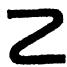
\includegraphics[keepaspectratio]{images/part003_0bad14cb.jpg}}

由命题 2 推出，有限个下半连续函数的下包络仍是下半连续的；但对无穷族下半连续函数的下包络，这一般不成立。例如，设 r 为任一有理数，\(f_{r}\) 表示在 r 处等于 0 而对一切实数 \(x \neq r\) 等于 1 的函数；诸 \(f_{r}\) 的下包络是函数 g，它对每个有理数等于 0，对每个无理数等于 1（``Dirichlet 函数''），而这个函数在无理点处不下半连续。

推论. 空间 X 上一族连续实值函数的上包络在 X 上下半连续。

在第九章，§ 1，第 6 节，命题 5 中我们将证明，若 X 是可一致化的（且仅在这种情形），这个命题的逆命题为真：可一致化空间上的每个下半连续函数是一族连续函数的上包络。

命题 3. 实值函数 \(f\) （定义在拓扑空间 \(\mathbf{X}\) 上）在一点 \(a \in \mathbf{X}\) 处下半连续，当且仅当 \(\liminf_{x \to a} f(x) = f(a)\) {[}或等价地，当且仅当 \(\liminf_{x \to a} f(x) \geqslant f(a)\) {]}。

该条件是必要的。因为对任意给定的 \(h < f(a)\) ，存在一个邻域 \(V\) （在 \(a\) 处），使得 \(h < f(x)\) 对一切 \(x \in V\) 成立；因此

\[
h \leqslant \inf _ {x \in \mathbf {V}} f (x) \leqslant \liminf _ {x \rightarrow a} f (x)
\]

（§ 5，第 6 节，公式 (12)），于是 \(f(a) \leqslant \liminf_{x \to a} f(x)\) 。该条件是充分的；因为若它成立，则对每个 \(h < f(a)\) 存在一个邻域 \(V\) （在 \(a\) 处），使得 \(h \leqslant \inf_{x \in V} f(x)\) ，从而 \(f\) 在 \(a\) 处下半连续。

命题 4. 设 \(f\) 是定义在子集 \(A\) （在拓扑空间 \(X\) 中稠密）上的任意实值函数。若对每个 \(x \in X\) 令 \(g(x) = \liminf_{y \to x, y \in A} f(y)\) ，则 \(g\) 在 \(X\) 上下半连续。

因为对任意给定的 \(h < g(x)\) ，存在一个开邻域 \(\mathbf{V}\) （在 \(x\) 处），使得对一切 \(z \in \mathbf{V} \cap \mathbf{A}\) 有 \(h < f(z)\) ；而 \(\mathbf{V}\) 是它的每个点 \(y\) 的邻域；于是 \(\liminf_{z \to y, z \in \mathbf{A}} f(z) = g(y) \geqslant h\) 对一切 \(y \in \mathbf{V}\) 成立，由此即得结果。

函数 g 称为 f 的下半连续正则化。~我们类似地定义 f 的上半连续正则化。

我们也可以把 \(g\) 定义为诸下半连续函数 \(\varphi\) （定义在 \(\mathbf{X}\) 上，且满足 \(\varphi(x) \leqslant f(x)\) 对一切 \(x \in \mathbf{A}\) 成立）中最大的一个。若 \(f\) 在 \(\mathbf{A}\) 上下半连续，则由命题 3，\(g\) 是 \(f\) 到 \(\mathbf{X}\) 的一个延拓。

\section{实数的无穷和与无穷乘积}

由于 \(\mathbf{R}\) 的每一点都有可数的基本邻域系（§ 1，第 4 节，命题 3 的推论），由此推出，有限实数的族 \((x_{t})\) 在 \(\mathbf{R}\) 中可和只当指标 \(t\) （满足 \(x_{t} \neq 0\) ）组成的集合是可数的（第三章，§ 5，第 2 节，命题 1 的推论）。于是 \(\mathbf{R}\) 中可和族的研究本质上归结为可和序列的研究。然而，以后我们不得不考虑不可数的有限实数族 \((x_{t})\) ，其各项是参数 \(t\) 的函数；可能发生这样的情形：对一切 t 该族可和，但由指标 \(\iota\) （满足 \(x_{t} \neq 0\) ）组成的（可数）集合依赖于 t。由于这个原因，下面我们对指标集的势不作任何假设。

\subsection{R 中可和的正有限数族}

定理 1. 族 \((x_{t})\) （由有限实数 \(\geqslant 0\) 组成）在 \(\mathbf{R}\) 中可和当且仅当该族的有限部分和组成的集合在 \(\mathbf{R}\) 中上有界。此时，该集合的上确界就是族 \((x_{t})\) 的和。

对指标集 I 的每个有限子集 H，令 \(s_{H} = \sum_{i \in H} x_{i}\) ；由于诸 \(x_{i}\) \(\geqslant 0\) ，关系 \(H \subset H'\) 蕴含 \(s_{H} \leqslant s_{H'}\) 。换句话说，映射 \(H \to s_{H}\) 是 I 的有限子集组成的有向集 \(\mathfrak{F}(I)\) 上的递增函数；因此（§ 5，第 2 节，定理 2 的推论）它有有限极限当且仅当它上有界。

注. 设 \((\mathrm{H}_{\lambda})\) 是 I 的有限子集的一个族，使得对 I 的每个有限子集 H，存在指标 \(\lambda\) 满足 \(H \subset H_{\lambda}\) ；则 \((x_{t})\) 可和当且仅当诸 \(s_{H_{1}}\) 组成的族在 R 中上有界。特别地，设 \((x_{n})\) 是有限实数 \(\geqslant 0\) 的序列，且对每个整数 n 令 \(s_{n} = \sum_{p=0}^{n} x_{p}\) ；则序列 \((x_{n})\) 在 R 中可和当且仅当对一个严格递增整数序列 \((n_{k})\) ，部分序列 \((s_{n_{k}})\) 在 R 中上有界。

例. 1) 对每个数 \(q\) （满足 \(0 \leqslant q < 1\) ），序列 \((q^n)\) （'公比为 \(q''\) 的等比数列'）在 \(\mathbf{R}\) 中可和，因为 \(s_n = \frac{1 - q^{n+1}}{1 - q} \leqslant \frac{1}{1 - q}\) ；该序列的和为 \(\lim_{n \to \infty} s_n = \frac{1}{1 - q}\) 。

\begin{enumerate}
\def\labelenumi{\arabic{enumi})}
\setcounter{enumi}{1}
\tightlist
\item
  设 \(a\) 与 \(b\) 是两个数，满足 \(0 \leqslant a < 1\) 与 \(0 \leqslant b < 1\) ；则族 \((a^{m}b^{n})_{(m,n) \in \mathbb{N} \times \mathbb{N}}\) 在 \(\mathbb{R}\) 中可和。因为 \(\mathbf{N} \times \mathbf{N}\) 的每个有限子集都含于形如 \([0, p] \times [0, p]\) 的子集，且我们有
\end{enumerate}

\[
\sum_ {m = 0} ^ {p} \sum_ {n = 0} ^ {p} a ^ {m} b ^ {n} = \left(\sum_ {m = 0} ^ {p} a ^ {m}\right) \left(\sum_ {n = 0} ^ {p} b ^ {n}\right) = \frac {1 - a ^ {p + 1}}{1 - a}. \frac {1 - b ^ {p + 1}}{1 - b} \leqslant \frac {1}{(1 - a) (1 - b)}.
\]

\begin{enumerate}
\def\labelenumi{\arabic{enumi})}
\setcounter{enumi}{2}
\tightlist
\item
  对每个整数 \(p > 1\) ，序列 \((n^{-p})\) ( \(n > 0\) )可和，因为
\end{enumerate}

\[
s _ {2 ^ {n + 1}} - s _ {2 ^ {n}} = \sum_ {k = 1} ^ {2 ^ {n}} (2 ^ {n} + k) ^ {- p} <   2 ^ {n}. (2 ^ {n}) ^ {- p}
\]

从而把这些不等式相加，得

\[
s _ {2 ^ {n}} <   \frac {1}{1 - 2 ^ {1 - p}}.
\]

\begin{enumerate}
\def\labelenumi{\arabic{enumi})}
\setcounter{enumi}{3}
\tightlist
\item
序列 \((1 / n)\) \((n > 0)\) 在 \(\mathbf{R}\) 中不可和，因为
\end{enumerate}

\[
s _ {2 ^ {n + 1}} - s _ {2 ^ {n}} = \sum_ {k = 1} ^ {2 ^ {n}} \frac {1}{2 ^ {n} + k} > \frac {2 ^ {n}}{2 ^ {n + 1}} = \frac {1}{2}
\]

从而把这些不等式相加，得

\[
s _ {2 ^ {n}} > n / 2
\]

故定理 1 的判别准则不满足。

\begin{enumerate}
\def\labelenumi{\arabic{enumi})}
\setcounter{enumi}{4}
\tightlist
\item
  设 \((\mathbf{I}_n)\) 是两两不相交的非空开区间的一个序列，它们都含于一个长度为有限数 \(l\) 的区间中。该族中有限个区间的长度之和 \(\leqslant l\) （§ 1，第 5 节），因此诸 \(\mathbf{I}_n\) 的长度组成的族在 \(\mathbf{R}\) 中可和，且其和 \(\leqslant l\) 。
\end{enumerate}

定理 2（比较原理）. 设 \((x_{\iota})_{\iota\in I}\) 与 \((y_{\iota})_{\iota\in I}\) 是有限实数 \(\geqslant 0\) 的两个族，满足 \(x_{\iota}\leqslant y_{\iota}\) 对一切 \(\iota\) 成立。若 \((y_{\iota})\) 在 \(\mathbb{R}\) 中可和，则 \((x_{\iota})\) 也可和，且我们有 \(\sum_{\iota}x_{\iota}\leqslant\sum_{\iota}y_{\iota}\) ；此外若存在指标 \(\chi\) 使 \(x_{\chi}<y_{\chi}\) ，则 \(\sum_{\iota}x_{\iota}<\sum_{\iota}y_{\iota}\) 。

假设蕴含

\[
\sum_ {\iota \in \mathbf {H}} x _ {\iota} \leqslant \sum_ {\iota \in \mathbf {H}} y _ {\iota},
\]

对 I 的每个有限子集 H 成立，定理的第一部分由此得证；关于和的不等式则由不等式延拓原理（§ 5，第 2 节，定理 1）得出。若 \(x_{\chi} < y_{\chi}\) ，则

\[
\sum_ {\iota} x _ {\iota} = x _ {\chi} + \sum_ {\iota \neq \chi} x _ {\iota} <   y _ {\chi} + \sum_ {i \neq x} y _ {\iota} = \sum_ {\iota} y _ {\iota}.
\]

这个定理提供了判断序列 \((x_{n})\) （由实数 \(\geqslant0\) 组成）在 R 中是否可和的最常用判别准则：我们设法把给定的序列与一个较简单的序列 \((y_{n})\) 相比较，后者的可和性我们已经知道。如果存在有限数 a \textgreater{} 0 ，使得从某个点起对一切 n 有 \(x_{n} \leqslant ay_{n}\) ，且 \((y_{n})\) 可和，则 \((x_{n})\) 可和；反之，如果存在有限数 b \textgreater{} 0 ，使得从某个点起对一切 n 有 \(x_{n} \geqslant by_{n}\) ，且 \((y_{n})\) 在 R 中不可和，则 \((x_{n})\) 在 R 中不可和。我们将在后续分册中看到，在最常出现的情形如何得到这样的比较序列。

例. 1) 设 \(a\) 是有限实数 \(>0\) ，考虑序列 \(\left(\frac{a^n}{n!}\right)\) ；设 \(n_0\) 是使 \(a < n_0\) 的最小整数。则

对每个 \(n \geqslant n_0\) 我们有

\[
\frac {a ^ {n}}{n !} \leqslant \frac {a ^ {n _ {0}}}{n _ {0} !} \cdot \left(\frac {a}{n _ {0}}\right) ^ {n - n _ {0}};
\]

由于 \(q = \frac{a}{n_0} < 1\) ，序列 \((q^{n - n_0})\) 可和，因此序列 \(\left(\frac{a^n}{n!}\right)\) 也可和。

\begin{enumerate}
\def\labelenumi{\arabic{enumi})}
\setcounter{enumi}{1}
\tightlist
\item
  设 \((a_{n})\) 是正数的一个可和序列。由于
\end{enumerate}

\[
\lim _ {n \rightarrow \infty} a _ {n} = 0,
\]

存在整数 \(n_0\) ，使得 \(a_n \leqslant 1\) 只要 \(n \geqslant n_0\) 。于是对每个 \(n \geqslant n_0\) 有 \(a_n^2 \leqslant a_n\) ，因此序列 \((a_n^2)\) 在 \(\mathbb{R}\) 中可和。序列 \((a_n^p)\) 对每个整数 \(p > 1\) 也可和。

\begin{enumerate}
\def\labelenumi{\arabic{enumi})}
\setcounter{enumi}{2}
\tightlist
\item
  设 \(a\) 与 \(b\) 是两个数 \(< 1\) ；则
\end{enumerate}

\[
\frac {1}{a ^ {m} + b ^ {n}} \leqslant \frac {1}{2 (\sqrt {a}) ^ {m} (\sqrt {b}) ^ {n}}
\]

因而族 \(\left(\frac{1}{a^m + b^n}\right)\) 在 \(\mathbf{R}\) 中可和。

推论. 设 \((x_{i})_{i\in I}\) 是 R 中有限数 \(\geqslant 0\) 的可和族。若 H 是 I 的任一子集，我们有

\[
\sum_ {i \in \mathbf {H}} x _ {i} \leqslant \sum_ {i \in \mathbf {I}} x _ {i},
\]

且等号仅当 \(x_{i} = 0\) 对一切 \(i \in \mathbb{C}\mathbb{H}\) 成立时才成立。

\subsection{R 中任意符号有限数的可和族}

定理 3. 设 \((x_{t})_{t\in I}\) 是有限实数的一个族；则下述命题等价：

\begin{enumerate}
\def\labelenumi{\alph{enumi})}
\item
  族 \((x_{i})\) 在 \(\mathbf{R}\) 中可和。
\item
  族 \((|x_{i}|)\) 在 \(\mathbf{R}\) 中可和。
\item
  族 \((x_{t})\) 的有限部分和组成的集合在 R 中有界。
\end{enumerate}

设 \(I_1\) 是所有 \(i \in I\) （满足 \(x_i \geq 0\) ）组成的集合，\(I_2\) 是所有 \(i \in I\) （满足 \(x_i < 0\) ）组成的集合。族 \((x_i)_{i \in I}\) {[}相应地，\((|x_i|)_{i \in I}\) {]}可和当且仅当族 \((x_i)_{i \in I_1}\) 与 \((x_i)_{i \in I_2}\) {[}相应地，\((|x_i|)_{i \in I_3}\) 与 \((|x_i|)_{i \in I_4}\) {]}中的每一个都可和（第三章，§ 5，第 3 节，命题 2 与命题 3）。而说 \((x_i)_{i \in I_1}\) 可和、或说 \((|x_i|)_{i \in I_2}\) 可和、或说族 \((x_{i})_{i\in I_1}\) 的有限部分和组成的集合有界（第 1 节，定理 1），这是一回事；把 \(I_1\) 换成 \(I_2\) ，同样的结论也成立。定理随即得出。

定理 3 表明，有限实数族在 R 中的可和性只依赖于其绝对值族的可和性。

我们回忆（第三章，§ 5，第 5 节，命题 6）：若 \((x_{t})\) 与 \((y_{t})\) 是有限实数的两个可和族，则族 \((x_{t} + y_{t})\) 可和，且 \(\sum_{i}(x_{t} + y_{t}) = \sum_{i}x_{t} + \sum_{i}y_{t}\) 。此外，若 \((x_{t})\) 是有限实数的可和族而 \(a\) 是任意有限实数，则族 \((ax_{t})\) 在 \(\mathbf{R}\) 中可和，且我们有 \(\sum_{i}ax_{t} = a\) . \(\sum_{i}x_{t}\) 。

\subsection{两个无穷和的乘积}

命题 1. 若有限实数的族 \((x_{\lambda})_{\lambda \in L}\) 与 \((y_{\mu})_{\mu \in M}\) 在 \(\mathbf{R}\) 中可和，则族 \((x_{\lambda}y_{\mu})_{(\lambda ,\mu)\in L\times M}\) 也可和，且我们有

\[
\sum_ {(\lambda , \mu) \in \mathbf {L} \times \mathbf {M}} x _ {\lambda} y _ {\mu} = (\sum_ {\lambda \in \mathbf {L}} x _ {\lambda}) (\sum_ {\mu \in \mathbf {M}} y _ {\mu}).\tag{1}
\]

\(\mathbf{L} \times \mathbf{M}\) 的每个有限子集都含于形如 \(\mathbf{H} \times \mathbf{K}\) 的有限子集，其中 \(\mathbf{H}\) 是 \(\mathbf{L}\) 的有限子集，\(\mathbf{K}\) 是 \(\mathbf{M}\) 的有限子集。根据假设，存在数 \(a > 0\) ，使得 \(\sum_{\lambda \in \mathbf{H}} |x_{\lambda}| \leqslant a\) 与 \(\sum_{\mu \in \mathbf{K}} |y_{\mu}| \leqslant a\) 对 \(\mathbf{H}\) 与 \(\mathbf{K}\) （\(\mathbf{L}\) 与 \(\mathbf{M}\) 的所有有限子集）分别成立；因此

\[
\sum_ {(\lambda , \mu) \in \mathbf {H} \times \mathbf {K}} | x _ {\lambda} y _ {\mu} | = (\sum_ {\lambda \in \mathbf {H}} | x _ {\lambda} |) (\sum_ {\mu \in \mathbf {K}} | y _ {\mu} |) \leqslant a ^ {2},
\]

而由定理 1 与定理 3，这表明族 \((x_{\lambda}y_{\mu})\) 在 \(\mathbf{R}\) 中可和。由结合律我们可以写{[}第三章，§ 5，第 3 节，公式 (2){]}

\[
\sum_ {(\lambda , \mu) \in \mathbf {L} \times \mathbf {M}} x _ {\lambda} y _ {\mu} = \sum_ {\lambda \in \mathbf {L}} (\sum_ {\mu \in \mathbf {M}} x _ {\lambda} y _ {\mu}) = \sum_ {\lambda \in \mathbf {L}} x _ {\lambda} (\sum_ {\mu \in \mathbf {M}} y _ {\mu}) = (\sum_ {\lambda \in \mathbf {L}} x _ {\lambda}) (\sum_ {\mu \in \mathbf {M}} y _ {\mu});
\]

由此即得结论。

\subsection{R* 中可乘的族}

在有限非零实数的乘法群 \(\mathbb{R}^*\) 中，族 \((x_{t})_{i\in I}\) 只当 \(\lim x_{t} = 1\) （关于 I 的有限子集的余集组成的滤子）时才可能可乘（第三章，§ 5，第 2 节，命题 1）。特别地，指标 \(i\) （使 \(x_{t} < 0\) ）只能有有限多个。因此我们可以限于只考虑各项都严格为正的族 \(x_{t}\) ；这时令 \(x_{i} = i + u_{i}\) 是方便的，其中诸 \(u_{i}\) 满足不等式 \(-i < u_{i} < +\infty\) （对一切 \(i\) ）。由于 \(\mathbf{R}^*\) 的每一点都有可数的基本邻域系，指标 \(i\) （使 \(u_{i} \neq 0\) ）组成的集合是可数的，只要族 \((i + u_{i})\) 在 \(\mathbf{R}^*\) 中可乘。

定理 4. 族 \((1 + u_{t})\) 在 \(\mathbb{R}^*\) 中可乘当且仅当族 \((u_{t})\) 在 \(\mathbb{R}\) 中可和。

引理. (i) 若 \((a_{i})_{1\leqslant i\leqslant p}\) 是数 \(>0\) 的一个有限序列，则

\[
\prod_ {i = 1} ^ {p} \left(1 + a _ {i}\right) \geqslant 1 + \sum_ {i = 1} ^ {p} a _ {i}.\tag{2}
\]

\begin{enumerate}
\def\labelenumi{(\roman{enumi})}
\setcounter{enumi}{1}
\tightlist
\item
  若又有 \(a_i < 1\) 对每个 \(i\) 成立，则
\end{enumerate}

\[
\prod_ {i = 1} ^ {p} \left(\mathrm{I} - a _ {i}\right) \geqslant \mathrm{I} - \sum_ {i = 1} ^ {p} a _ {i}.\tag{3}
\]

这些不等式当 \(p = 1\) 时是显然的，并可对 \(p\) 用归纳法证明。若

\[
\prod_ {i = 1} ^ {p - 1} \left(\mathrm{I} + a _ {i}\right) \geqslant \mathrm{I} + \sum_ {i = 1} ^ {p - 1} a _ {i},
\]

则我们有

\[
\prod_ {i = 1} ^ {p} \left(\mathrm{I} + a _ {i}\right) \geqslant \left(\mathrm{I} + a _ {p}\right) \left(\mathrm{I} + \sum_ {i = 1} ^ {p - 1} a _ {i}\right) = \mathrm{I} + \sum_ {i = 1} ^ {p} a _ {i} + a _ {p}. \sum_ {i = 1} ^ {p - 1} a _ {i} \geqslant \mathrm{I} + \sum_ {i = 1} ^ {p} a _ {i}.
\]

同样，若

\[
\prod_ {i = 1} ^ {p - 1} \left(\mathrm{I} - a _ {i}\right) \geqslant \mathrm{I} - \sum_ {i = 1} ^ {p - 1} a _ {i},
\]

则我们有

\[
\prod_ {i = 1} ^ {p} \left(\mathrm{I} - a _ {i}\right) \geqslant \left(\mathrm{I} - a _ {p}\right) \left(\mathrm{I} - \sum_ {i = 1} ^ {p - 1} a _ {i}\right) = \mathrm{I} - \sum_ {i = 1} ^ {p} a _ {i} + a _ {p}. \sum_ {i = 1} ^ {p - 1} a _ {i} \geqslant \mathrm{I} - \sum_ {i = 1} ^ {p} a _ {i}.
\]

证明了引理之后，我们注意，若族 \((\mathbf{I} + u_{t})\) 可乘，则族 \((\mathbf{I} + u_{t}^{+})\) 与 \((\mathbf{I} - u_{t}^{-})\) 也可乘，因为 \(\mathbf{R}^*\) 是完备群（第三章，§ 5，第 3 节，命题 2）；反之，若族 \((\mathbf{I} + u_{t}^{+})\) 与 \((\mathbf{I} - u_{t}^{-})\) 可乘，则 \((\mathbf{I} + u_{t})\) 也可乘（第三章，§ 5，第 3 节，命题 3）。因此我们只需考虑两种情形：一切 \(u_{t}\) 都 \(\geqslant 0\) ，或它们都 \(\leqslant 0\) 。

首先设 \(u_{t} \geqslant 0\) 对一切 \(t\) 成立。若族 \((1 + u_{t})\) 可乘，则对每个 \(\varepsilon > 0\) ，存在一个有限子集 \(J\) （属于指标集 \(I\) ），使得对每个有限子集 \(H\) （含于 \(I\) 且与 \(J\) 不相交），有 \(\mathbf{I} \leqslant \prod_{i \in \mathbf{H}} (\mathbf{I} + u_i) \leqslant \mathbf{I} + \varepsilon\) ；由 (2) 推出 \(\sum_{i \in \mathbf{H}} u_i \leqslant \varepsilon\) ，这表明由 Cauchy 判别准则（第三章，§ 5，第 2 节，定理 I），\((u_i)\) 在 \(\mathbf{R}\) 中可和。

反之，设 \((u_{t})\) 在 \(\mathbf{R}\) 中可和。对每个 \(\varepsilon\) （满足 \(0 < \varepsilon < 1\) ），存在一个有限子集 \(J\) （\(I\) 的），使得对每个有限子集 \(H\) （含于 \(I\) 且与 \(J\) 不相交），有 \(0 \leqslant \sum_{t \in H} u_{t} \leqslant \varepsilon\) 。由 (3)，我们因此有 \(\prod_{t \in H} (I - u_{t}) \geqslant I - \varepsilon\) ；但由于 \(I + u \leqslant \frac{I}{I - u}\) 对每个数 \(u\) （满足 \(0 \leqslant u < 1\) ）成立，由此推出

\[
\mathrm{I} \leqslant \prod_ {i \in \mathrm{H}} (\mathrm{I} + u _ {i}) \leqslant \frac {\mathrm{I}}{\mathrm{I} - \varepsilon},
\]

而这表明 \((\mathbf{I} + u_{t})\) 可乘（Cauchy 判别准则）。

当一切 \(u_{i}\) 都 \(\leqslant 0\) 时证明类似。为证明 \((u_{i})\) 可和当 \((1 + u_{i})\) 可乘，用公式 (2) 及不等式 \(1 - u \leqslant \frac{1}{1 + u}\) ( \(0 \leqslant u < 1\) )；为证明 \((1 + u_{i})\) 可乘当 \((u_{i})\) 可和，用公式 (3)。

在第五章（§ 4）中，群 \(\mathbf{R}^*\) 的拓扑研究将使我们能借助对数函数给出族在 \(\mathbf{R}^*\) 中可乘的另一个判别准则；在后续分册中我们将利用对数的微分性质证明这个判别准则与上面那个等价。

\subsection{\texorpdfstring{\(\overline{\mathbf{R}}\) 中的可和族与可乘族}{SUMMABLE FAMILIES AND MULTIPLIABLE FAMILIES IN \textbackslash overline\{\textbackslash mathbf\{R\}\}}}

在区间 \([0, +\infty]\) （\(\overline{\mathbf{R}}\) 中的）上，加法是一个结合的、交换的合成法则（§ 4，第 3 节）；因此在该区间中数的可和族的概念已有定义（第三章，§ 5，第 1 节，注 3）。

命题 2. 族 \((x_{\mathfrak{t}})\) （由实数 \(\geqslant 0\) 组成）的每一个在 \(\overline{\mathbf{R}}\) 中可和。因为映射 \(\mathbf{H} \to s_{\mathbf{H}}\) （由有向集 \(\mathfrak{F}(\mathbf{I})\) 到 \(\overline{\mathbf{R}}\) 中）是递增的；故（§ 5，第 2 节，定理 2）有极限。

同样的推理表明，实数 \(\leqslant 0\) 的每个族在 \(\overline{\mathbf{R}}\) 中可和。

类似地，乘法在区间 \([0, 1]\) 与 \([1, +\infty]\) （\(\overline{R}\) 中的）的每一个上都是一个结合的、交换的合成法则，因此可乘族的概念在每个这样的区间上都有定义。

命题 3. 每个族 \((1 + u_{t})\) {[}相应地，\((1 - u_{t})]\) ——由数 \(\geqslant 1\) （相应地，\(\geqslant 0\) 且 \(\leqslant 1\) ）组成——在 \(\overline{\mathbf{R}}\) 中可乘。

与命题 2 的证明相同。

推论. 积 \(\prod_{i} (1 + u_i) [\text{resp. } \prod_{i} (1 - u_i))\) （由数 \(\geqslant 1\) （相应地，\(>0\) 且 \(\leqslant 1\) ）组成）等于 \(+\infty\) （相应地，0）当且仅当 \(\sum_{i} u_i = +\infty\) 。因为若 \(\sum_{i} u_i\) 有限，则 \(\prod_{i} (1 + u_i)\) 与 \(\prod_{i} (1 - u_i)\) 属于 \(\mathbf{R}^*\) ，反之亦然（第 4 节，定理 4）。

注. 结合性定理（第三章，§ 5，第 3 节，定理 2）当把 G 换成 \(\overline{\mathbf{R}}\) 并假设诸 \(x_{i}\) \(\geqslant 0\) 时仍然成立。若 \(\sum_{i \in I} x_{i}\) 有限，这是显然的。反之设 \(\sum_{i \in I} x_{i} = +\infty\) 。则对每个有限的 \(a > 0\) ，存在 I 的有限子集 H 使得 \(\sum_{i \in H} x_{i} \geqslant a\) 。设 K 是 L 的有限子集且 \(H \subset \bigcup_{\lambda \in K} I_{\lambda}\) ；那么由于 \(s_{\lambda} \geqslant \sum_{i \in I_{\lambda} \cap H} x_{i}\) 对一切 \(\lambda \in K\) ，我们有

\[
\sum_ {\lambda \in \mathbf {K}} s _ {\lambda} \geqslant \sum_ {i \in \mathbf {H}} x _ {i} \geqslant a,
\]

这表明 \(\sum_{\lambda \in L} s_{\lambda} = +\infty\) 。我们把对 \([0, 1]\) 或 \([1, +\infty]\) 中的数的可乘族表述类似命题的任务留给读者。

\subsection{实数的无穷级数与无穷乘积}

有限实数的级数，若它在 R 中收敛，就简称为收敛的。

定义 1. 有限实数的级数称为绝对收敛的，如果其各项的绝对值组成的级数收敛。

命题 4. 有限实数的级数交换收敛当且仅当它绝对收敛。

这由第三章，§ 5，第 7 节，命题 9 以及第 2 节的定理 3 得出。

换句话说，若 \((u_{n})\) 是有限实数的序列，则说通项为 \(u_{n}\) 的级数交换收敛、或说它绝对收敛、或说序列 \((u_{n})\)

在 \(\mathbf{R}\) 中可和，这是一回事。于是第三章 § 5 中证明的可和族的一切性质都可应用于绝对收敛级数。特别地，若通项为 \(u_{n}\) 的级数绝对收敛，则和 \(\sum_{n\in\mathbf{H}} u_{n}\) 对子集 \(\mathbf{H}\) （\(\mathbf{N}\) 的所有子集）存在；又若 \((\mathbf{H}_{p})\) 是 \(\mathbf{N}\) 的一个分拆，我们有

\[
\sum_ {n = 0} ^ {\infty} u _ {n} = \sum_ {p} \left(\sum_ {n \in \mathrm{H} _ {p}} u _ {n}\right)
\]

（绝对收敛级数的结合性）。

正如我们已在第三章 § 5 中指出的，实数级数可以收敛而不交换收敛，即不绝对收敛。

例. 交错级数. 由有限实数的序列 \((u_n)\) 定义的级数称为交错的，如果 \(u_n = (-1)^n v_n\) ，其中 \(v_n \geqslant 0\) 对一切 \(n\) 成立。我们来证明，这类级数收敛的一个充分条件是序列 \((v_n)\) 递减且以 \(0\) 为其极限。因为若 \(s_n\) 表示

\[
\sum_ {p = 0} ^ {n} u _ {p},
\]

\((v_{n})\) 递减这一假设蕴含

\[
s _ {2 n + 1} \leqslant s _ {2 n + 3} \leqslant s _ {2 n + 2} \leqslant s _ {2 n}
\]

对一切 \(n \geqslant 0\) 。序列 \((s_{2n})\) {[}相应地，\((s_{2n+1})\) {]}递减且下有界（相应地，递增且上有界），因此有有限极限 a（相应地，b），且 \(b \leqslant a\) ；由于

\[
a - b = \lim _ {n \rightarrow \infty} (s _ {2 n} - s _ {2 n + 1}) = \lim _ {n \rightarrow \infty} v _ {2 n + 1} = 0,
\]

断言得证。

例如若取 \(v_{n}=1/n\) ，上述条件满足，因此通项为 \((-1)^{n}/n\) 的级数（``交错调和级数''）收敛。我们在第 1 节已看到，通项为 1/n 的级数（``调和级数''）不收敛，从而交错调和级数不绝对收敛。

我们回忆（第三章，§ 5，第 6 节，命题 7）：若 \((u_n)\) 与 \((v_n)\) 是有限实数的两个收敛级数，则级数 \((u_n + v_n)\) 收敛，且

\[
\sum_ {n = 0} ^ {\infty} \left(u _ {n} + v _ {n}\right) = \sum_ {n = 0} ^ {\infty} u _ {n} + \sum_ {n = 0} ^ {\infty} v _ {n};
\]

又，若级数 \((u_{n})\) 收敛，则级数 \((au_{n})\) 对一切有限实数 \(a\) 收敛，且 \(\sum_{n=0}^{\infty} au_{n} = a\) . \(\sum_{n=0}^{\infty} u_{n}\) 。

最后，若级数 \((u_n)\) 与 \((v_n)\) 收敛，且 \(u_n \leqslant v_n\) 对一切 \(n\) ，则由不等式延拓原理（§ 5，第 2 节，定理 1），\(\sum_{n=0}^{\infty} u_n \leqslant \sum_{n=0}^{\infty} v_n\) 。

应当注意，若设级数 \((v_{n})\) 收敛但不绝对收敛，且对每个 n 有 \(|u_{n}| \leqslant |v_{n}|\) ，我们决不能推断级数 \((u_{n})\) 收敛，取 \(u_{n} = |v_{n}|\) 即见。

有限非零实数的无穷乘积，若它在 \(\mathbf{R}^*\) 中收敛，就简称为收敛的；此时它的值是有限的非零实数。

定义 2. 通项因子为 \(1 + u_{n}\) 的无穷乘积称为绝对收敛的，如果通项因子为 \(1 + |u_{n}|\) 的乘积收敛。

命题 5. 有限实数的无穷乘积交换收敛当且仅当它绝对收敛。

这由第三章，§ 5，第 7 节，命题 9 以及上面的定理 4 得出。

此外，通项因子为 \(1 + u_{n}\) 的乘积绝对收敛当且仅当通项为 \(u_{n}\) 的级数绝对收敛。

非零实数的乘积可以收敛而不交换收敛，即不绝对收敛。

例. 若取 \(u_{2n-1} = -\frac{1}{n}\) 与 \(u_{2n} = \frac{1}{n}\) （对 \(n \geqslant 2\) ），则乘积 \((1 + u_n)\) 不绝对收敛，因为级数 \((u_n)\) 不绝对收敛；但由于

\[
\begin{array}{l} \prod_ {p = 3} ^ {n} (1 + u _ {p}) = \prod_ {p = 2} ^ {n} \left(1 - \frac {1}{p ^ {2}}\right), \\ \text { and } \quad \prod_ {p = 3} ^ {2 n + 1} (1 + u _ {p}) = \left(1 - \frac {1}{n + 1}\right) \prod_ {p = 2} ^ {n} \left(1 - \frac {1}{p ^ {2}}\right), \end{array}
\]

由定理 4 推出该乘积收敛，且其值为

\[
\prod_ {n = 2} ^ {\infty} \left(1 - \frac {1}{n ^ {2}}\right).
\]

\pandocbounded{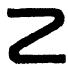
\includegraphics[keepaspectratio]{images/part003_4cdcc444.jpg}}

此外应当指出，通项为 \(u_{n}\) 的级数的收敛性对于通项因子为 \(1 + u_{n}\) 的乘积的收敛性既不必要也不充分（见习题 21 与 22）。

\section{实数的通常展开；R 的势}

\subsection{实数的近似}

定义 1. 给定一个数 \(\varepsilon > 0\) ，实数 \(r\) 称为精确到 \(\varepsilon\) 的实数 \(x\) 的近似，如果 \(|x - r| \leqslant \varepsilon\) ；\(r\) 称为不足近似，如果 \(r \leqslant x\) ；称为过剩近似，如果 \(r \geqslant x\) 。

设 A 是 R 的一个稠密子集。对每个 \(x \in R\) 与每个 \(\varepsilon > 0\) ，存在 x 的属于 A 的精确到 \(\varepsilon\) 的不足（相应地，过剩）近似，因为区间 \(]x - \varepsilon, x[\) （相应地，\(]x, x + \varepsilon[\) ）至少含有 A 的一个点。现在若考虑一个给定的严格递减序列 ( \(\varepsilon_{n}\) ) （由数 \textgreater{} 0 组成，趋于 0），而 \(r_{n}\) 是 x 的精确到 \(\varepsilon_{n}\) 的近似，则序列 ( \(r_{n}\) ) 当 n 趋于无穷时以 x 为极限。

在 A 是加法群 R 的子群且限制 \(\varepsilon_{n}\) 属于 A 的情形，我们对每个 \(x \in R\) 都能按典型方式定义一个由 x 的属于 A 的不足近似组成的序列 \((r_{n})\) 。

因为由 Archimedes 公理（§ 2，第 1 节，定理 1），整数 \(p\) （满足 \(p\varepsilon_n \leqslant x\) ）组成的集合有一个最大元 \(p_n\) ；换言之，存在唯一的整数 \(p_n\) 使得

\[
p _ {n} \varepsilon_ {n} \leqslant x <   (p _ {n} + 1) \varepsilon_ {n}.\tag{1}
\]

由于 \(|x - p_n\varepsilon_n| \leqslant \varepsilon_n\) ，由此推出 \(p_n\varepsilon_n\) 是 \(x\) 的精确到 \(\varepsilon_n\) 的不足近似，且由假设属于 A；类似地，\((p_n + 1)\varepsilon_n\) 是 \(x\) 的属于 A 的精确到 \(\varepsilon_n\) 的过剩近似，而两个序列 \((p_n\varepsilon_n)\) 与 \(((p_n + 1)\varepsilon_n)\) 都以 \(x\) 为极限。

\subsection{实数关于基序列的展开}

我们将限于研究 \(\varepsilon_{n} = 1 / d_{n}\) 的情形，其中 \((d_n)\) 是整数的一个严格递增序列，满足 \(d_0 = 1\) ，且 \(d_n\) 是 \(d_{n-1}\) 的倍数（对 \(n \geqslant 1\) ）。令 \(a_n = d_n / d_{n-1}\) ( \(n \geqslant 1\) )：\(a_n\) 是一个整数 \(>1\) 。在这种情形，不足近似 \(r_n = p_n / d_n\) 组成的序列是递增的，因为 \(p_n\) 是使 \(p_n / d_n \leqslant x\) 成立的最大整数；

但我们有

\[
\frac {p _ {n - 1}}{d _ {n - 1}} = \frac {p _ {n - 1} a _ {n}}{d _ {n}} \leqslant x <   \frac {p _ {n - 1} + 1}{d _ {n - 1}} = \frac {p _ {n - 1} a _ {n} + a _ {n}}{d _ {n}}
\]

于是 \(a_{n}p_{n - 1}\leqslant p_{n} <   a_{n}p_{n - 1} + a_{n},\) ，因此 \(r_{n - 1}\leqslant r_n\leqslant x.\) 令

\[
p _ {n} = a _ {n} p _ {n - 1} + u _ {n};\tag{2}
\]

则 \(0 \leqslant u_n < a_n\) ，它等价于 \(0 \leqslant u_n \leqslant a_n - 1\) ，因为 \(u_n\) 是整数。由此

\[
r _ {n} = r _ {n - 1} + \frac {u _ {n}}{d _ {n}} = p _ {0} + \sum_ {k = 1} ^ {n} \frac {u _ {k}}{d _ {k}},\tag{3}
\]

并且，由于 \(x = \lim_{n\to \infty}r_n,\)

\[
x = p _ {0} + \sum_ {n = 1} ^ {\infty} \frac {u _ {n}}{d _ {n}}.\tag{4}
\]

(4) 右端的级数，其和为 \(x\) ，称为 \(x\) 关于基序列 \((d_n)\) 的展开。所有系数 \(u_n\) 都 \(\geqslant 0\) ；\(p_0\) 依定义是最大整数 \(p\) （满足 \(p \leqslant x\) ）；它称为 \(x\) 的整数部分，常记作 {[}x{]}。

\subsection{用展开式定义实数}

反之，设给定了一个整数 \(q_0\) 与整数的序列 \((v_n)\) ( \(n \geqslant 1\) )（满足 \(0 \leqslant v_n \leqslant a_n - 1\) ）；我们问是否存在一个数 \(x\) ，其展开 (4) 满足 \(p_0 = q_0\) 且 \(u_n = v_n\) 对一切 \(n\) 。如果这样的数存在，它就是唯一的，因为它等于 \(q_0 + \sum_{n=1}^{\infty} \frac{v_n}{d_n}\) 。

对每个整数 \(m > 0\) 我们有（由比较原理）

\[
\sum_ {n = m + 1} ^ {\infty} \frac {v _ {n}}{d _ {n}} \leqslant \sum_ {n = m + 1} ^ {\infty} \frac {a _ {n} - 1}{d _ {n}} = \sum_ {n = m + 1} ^ {\infty} \left(\frac {1}{d _ {n - 1}} - \frac {1}{d _ {n}}\right) = \frac {1}{d _ {m}}
\]

而且最左端与最右端的项仅当 \(v_{n} = a_{n} - 1\) （对每个 \(n > m\) ）时才相等（§ 7，第 1 节，定理 2）。因此通项为 \(\frac{v_n}{d_n}\) 的级数收敛；此外，若 \(x = q_0 + \sum_{n=1}^{\infty} \frac{v_n}{d_n}\) ，我们有

\[
s _ {m} = q _ {0} + \sum_ {n = 1} ^ {m} \frac {v _ {n}}{d _ {n}} \leqslant x \leqslant s _ {m} + \frac {1}{d _ {m}}
\]

且 \(x = s_m + \frac{1}{d_m}\) 仅当 \(v_n = a_n - 1\) （对每个 \(n > m\) ）时成立。由于 \(s_m\) 是分母为 \(d_m\) 的分数，不足近似 \(r_m\) （它对 \(x\) 精确到 \(1/d_m\) ）等于 \(s_m\) 或 \(s_m + \frac{1}{d_m}\) ；且后一情形仅当 \(v_{n} = a_{n} - 1\) （对一切 \(n > m\) ）时才能发生。于是：

\begin{enumerate}
\def\labelenumi{(\roman{enumi})}
\item
  存在无穷多个 \(n\) 的值（满足 \(v_{n} < a_{n} - 1\) ）：这时级数 \(q_{0} + \sum_{n=1}^{\infty} \frac{v_{n}}{d_{n}}\) 与其和 \(x\) 的展开完全相同。
\item
  存在一个整数 \(m \geqslant 0\) 使得 \(v_{n} = a_{n} - 1\) （只要 \(n > m\) ），且 \(v_{m} < a_{m} - 1\) （若 \(m > 0\) ）；这时 \(x\) （级数 \(q_{0} + \sum_{n=1}^{\infty} \frac{v_{n}}{d_{n}}\) 的和）等于有理数
\end{enumerate}

\[
q _ {0} + \sum_ {n = 1} ^ {m} \frac {v _ {n}}{d _ {n}} + \frac {1}{d _ {m}}\tag{5}
\]

它是 \(k/d_{m}\) 型的（k 为整数）；x 的展开与级数 (5) 完全相同，其中所有指标 \textgreater{} m 的项都是零；这样的展开称为是有限的，或说是终止的。级数

\[
q _ {0} + \sum_ {n = 1} ^ {\infty} \frac {v _ {n}}{d _ {n}} = q _ {0} + \sum_ {n = 1} ^ {m} \frac {v _ {n}}{d _ {n}} + \sum_ {n = m + 1} ^ {\infty} \frac {a _ {n} - 1}{d _ {n}}\tag{6}
\]

称为数 x 的非正常展开。

反之，设 x 是一个有理数，它对 n 的某个值可以写成分母为 \(d_{n}\) 的分数。~设 m 是使 x 为 \(k/d_{m}\) 型（k 为整数）的最小整数；我们有 \(r_{n}<x\) （对 n\textless m），且 \(r_{m}=x\) ，因此 x 的展开具有形式 (5)，且 x 有一个由 (6) 给出的非正常展开；此外这个非正常展开是唯一的。

一个有理数，写成既约形式 \(p / q\) ，等于分母为 \(d_n\) 的分数当且仅当 \(q\) 整除 \(d_n\) （数 \(m\) 因而是这样的最小整数 \(n\) ：\(q\) 整除 \(d_n\) ）。可能发生这样的情形：每个有理数都具有这一性质（对适当选取的 \(n\) ）；当且仅当每个整数 \(> 0\) 整除某个 \(d_n\) （例如 \(d_n = n!\) ）时才是这种情形。如果诸 \(d_n\) 具有这一性质，那么一个数是有理数当且仅当它关于序列 \((d_n)\) 的展开终止。

概括起来：对每个序列 \(s\) ，其首项 \(q_{0}\) 是任意整数，且其项 \(v_{n}(n \geqslant 1)\) 满足 \(0 \leqslant v_{n} \leqslant a_{n} - 1\) ，对应着一个等于 \(q_{0} + \sum_{n=1}^{\infty} \frac{v_{n}}{d_{n}}\) 的实数；若 \(I_{n}\) 表示区间 \([0, a_{n} - 1]\) （\(N\) 中的），我们就这样定义了一个映射 \(\varphi\) （从 \(X = Z \times \prod_{n=1}^{\infty} I_{n}\) 到直线 \(R\) 上）；此外，方程 \(\varphi(s) = x\) ——其中 \(x \in R\) 已给定——当 \(x\) 不是分母为 \(d_{n}\) （对某个 \(n\) ）的分数时有一个解，否则有两个解。

\subsection{展开式的比较}

如果我们知道两个不同实数 \(x\) 与 \(y\) 的展开，就能判定是 \(x < y\) 还是 \(x > y\) 。

设 \(x = p_0 + \sum_{n=1}^{\infty} u_n / d_n\) ，\(y = q_0 + \sum_{n=1}^{\infty} v_n / d_n\) 是 \(x\) 与 \(y\) 的展开。若 \(p_0 < q_0\) 则 \(x < y\) ，因为

\[
p _ {0} \leqslant x <   p _ {0} + 1 \leqslant q _ {0} \leqslant y.
\]

更一般地，设 \(p_0 = q_0\) 且 \(u_n = v_n\) （对 \(1 \leqslant n \leqslant m\) ），但 \(u_m < v_m\) ；如果

\[
r _ {n} = p _ {0} + \sum_ {k = 1} ^ {n} u _ {k} / d _ {k}, \quad s _ {n} = q _ {0} + \sum_ {k = 1} ^ {n} v _ {k} / d _ {k},
\]

则 \(r_n = s_n\) （对 \(n < m\) ），且由于 \(u_m + 1 \leqslant v_m\) ，有 \(r_m + \frac{1}{d_m} \leqslant s_m\) ；但 \(r_m \leqslant x < r_m + \frac{1}{d_m} \leqslant s_m \leqslant y\) ，因此再次有 \(x < y\) 。换言之，\(x\) 与 \(y\) 的次序同于它们各自的展开中头两个不同项的次序。

由此推出，若 \(p_{0}=q_{0}\) 且 \(u_{n}=v_{n}\) （对 n\textless m），则每个属于以 x 与 y 为端点的闭区间的数 z 的展开的前 m 项与 x 与 y 的展开的前 m 项相同。

我们还注意，在这种情形有 \(|y - x| \leqslant \frac{1}{d_{m-1}}\) 。如果我们赋予

Z 与诸区间 \(I_{n}\) 以离散拓扑，则由此推出上面定义的映射 \(\varphi\) 在乘积空间 X 上连续。

\subsection{以 a 为底的展开}

最重要的基序列是那些 \(d_{n}=a^{n}\) 的序列，其中 a 是整数 \textgreater1；这时 a 称为相应展开的底数（或简称底）。对于数值计算，使用以 10 为底的展开，称为十进展开；以 2 为底（二进展开）与以 3 为底（三进展开）的展开也常被使用。

为了表示不足近似 \(r_n\) （对数 \(x \geqslant 0\) ，在其以 \(a\) 为底的展开中），采用下述记号：每个整数 \(u\) （满足 \(0 \leqslant u \leqslant a - 1\) ）用一个特定的记号表示；如果

\[
r _ {n} = p _ {0} + \sum_ {k = 1} ^ {n} \frac {u _ {k}}{d _ {k}},
\]

我们首先借助这些记号写出以 \(a\) 为底的整数 \(p_{0}=[x]\geqslant0\) 的表示（集合论，第三章，§ 5，第 7 节），然后放一个点（``小数点''），并写出

相继地表示数 \(u_1, u_2, \ldots, u_n\) 的记号。如果 \(S\) 是这样得到的符号，习惯上（滥用语言）写 \(x = S \ldots\) 。应当一劳永逸地理解：这样的关系式只是指示右端是 \(x\) 的精确到 \(1/a^n\) 的不足近似的一种缩写方法。

对于负数，通行习惯不同：我们用上述记号写出 \(x' = -x > 0\) 的一个近似，并在其前放置符号``-''；因此这样记的是 \(x\) 的精确到 \(1/a^n\) 的过剩近似。

这个用法对数值计算有其不便之处。在负对数的记号中，采用与正数相同的记号，而在整数部分上放一横杠，以指示它等于所写数的相反数。

\subsection{R 的势}

我们有 \(\mathbf{R} = \bigcup_{n\in \mathbf{Z}}[n,n + 1[,\) 且所有区间 \([n,n + 1[\) 都与 \([0,1[\) 等势。由于 \([0,1[\) 是无限集，由此推出 \(\mathbf{R}\) 与区间 \([0,1[\) 等势。通过考虑区间 \([0,1[\) 中数的二进展开，我们将证明这个区间与由每一项都等于 0 或 1 的序列 \((u_n)\) 组成的集合 S 等势。

首先，它与子集 \(S'\) （\(S\) 的，由序列 \((u_n)\) （满足 \(u_n = 0\) ，对无穷多个 \(n\) 的值）组成）等势。另一方面，余集 \(S''\) （\(S'\) 在 \(S\) 中的）与等于分母为 \(2^n\) 的分数的有理数的所有非正常展开组成的集合等势；这些数构成 \(Q\) 的一个子集，因此它们组成的集合是可数的，从而 \(S''\) 也是可数的。由于 \(S'\) 是无限的，它与 \(S\) 等势，由此即得结果。

现在 S 与 \(\mathfrak{P}(\mathbf{N})\) 等势；因为我们可以定义 \(\mathfrak{P}(\mathbf{N})\) 到 S 上的一个双射，把 N 的每个子集 A 映为序列 \((u_n)\) ，其中 \(u_n = 0\) 若 \(n \in A\) ，而 \(u_n = 1\) 若 \(n \in \mathbb{C}A\) 。我们这样就证明了：

定理 1（Cantor）. 实数组成的集合与一个可数无限集的一切子集组成的集合等势。

推论. 实数组成的集合的势严格大于可数集的势。

与 R 等势的集合称为具有连续统的势。由 § 4 第 1 节命题 1，每个含有多于一个点的区间都具有连续统的势。同样，R 的可数子集的余集具有连续统的势；特别地，所有无理数组成的集合具有连续统的势。

\BourbakiExercises
\BourbakiExerciseGroup

\begin{enumerate}
\def\labelenumi{\arabic{enumi})}
\tightlist
\item
  一个拓扑 \(\mathfrak{G}\) （在有序交换群 \(\mathbf{G}\) 上）称为与 \(\mathbf{G}\) 的序群结构相容，如果它与 \(\mathbf{G}\) 的群结构相容，此外集合 \(\mathbf{G}_{+}\) （由元素 \(x \geqslant 0\) （属于 \(\mathbf{G}\) ）组成）关于 \(\mathfrak{G}\) 是闭的。
\end{enumerate}

\begin{enumerate}
\def\labelenumi{\alph{enumi})}
\item
  设 \(\mathfrak{G}\) 是与 \(\mathbf{G}\) 的序群结构相容的一个 Hausdorff 拓扑，又设 \(\hat{\mathbf{G}}\) 是 \(\mathbf{G}\) 的完备化（关于 \(\mathfrak{G}\) ）。在群 \(\hat{\mathbf{G}}\) 中，闭包 \(\mathbf{P}\) （\(\mathbf{G}_{+}\) 的）是这样的：\(y - x \in \mathbf{P}\) 是一个与 \(\hat{\mathbf{G}}\) 的群结构相容的预序。
\item
  设 \(\theta\) 是一个无理数，考虑 \(\mathbf{Q}^2\) 上的这样一个序：其正元素组成的集合由 (0, 0) 与所有偶 \((x, y)\) （满足 \(y - \theta x \geqslant 0\) ）组成。关于这个序，\(\mathbf{Q}^2\) 是一个全序群，而 \(\mathbf{Q}^2\) 上由有理直线的拓扑与自身的乘积给出的拓扑与这个序群结构相容。但在 \(\hat{\mathbf{G}} = \mathbb{R}^2\) 上，关系 \(y - x \in \mathbf{P} = \overline{\mathbf{G}}_+\) 不是序。
\item
  在全序群 G 上，拓扑 \(\mathfrak{C}_{0}(\mathbf{G})\) （第一章，§ 2，习题 5）是与序群结构相容的所有拓扑中最粗的（区分两种情形，视所有 \(x > 0\) 组成的集合有还是没有最小元素而定）。G 上与 G 的群结构相容且细于 \(\mathfrak{C}_{0}(\mathbf{G})\) 的每个拓扑都与 G 的序群结构相容，且映射 \(x \to x^{+}\) 关于这样的拓扑连续。这个映射关于 \(\mathfrak{C}_{0}(\mathbf{G})\) 一致连续，但不一定关于一个群拓扑 \(\mathfrak{C}\) （严格细于 \(\mathfrak{C}_{0}(\mathbf{G})\) ）一致连续{[}见 b){]}。
\end{enumerate}

\begin{enumerate}
\def\labelenumi{\arabic{enumi})}
\setcounter{enumi}{1}
\tightlist
\item
  \begin{enumerate}
  \def\labelenumii{\alph{enumii})}
  \tightlist
  \item
    设 G 是一个格序交换群。对 G 中每个 \(x \geqslant 0\) ，令 \(\mathbf{I}(x)\) 表示 G 中的区间 \([-x, x]\) 。G 的一个非空族 \((c_{\alpha})\) （由元素 \(\geqslant 0\) 组成）使得诸区间 \(\mathbf{I}(c_{\alpha})\)
  \end{enumerate}
\end{enumerate}

构成 G 上与 G 的群结构相容的拓扑 \(\mathfrak{G}\) 在点 0 处的基本邻域系，当且仅当 \(c_{\alpha}\) 组成的集合是有向的（关于关系 \(\geqslant\) ），且对每个 \(\alpha\) 存在 \(\beta\) 使 \(2c_{\beta} \leqslant c_{\alpha}\) 。如果这些条件满足，G 到 G 中的映射 \(x \to x^{+}\) 一致连续。\(\mathfrak{G}\) 是 Hausdorff 的当且仅当 \(\inf c_{\alpha} = 0\) ；且在这种情形 \(\mathfrak{G}\) 与 G 的序群结构相容。

\begin{enumerate}
\def\labelenumi{\alph{enumi})}
\setcounter{enumi}{1}
\item
  在群 \(G = Z^{N}\) （可数无穷多个全序群 Z 的乘积）上，没有用 a) 的程序定义的非离散拓扑，但诸因子 Z 上的离散拓扑的乘积是 G 上的一个拓扑，它与 G 的序群结构相容，它是 Hausdorff 的且非离散的。
\item
  在全序群 G 上，用 a) 的程序定义的唯一 Hausdorff 拓扑是拓扑 \(\mathcal{G}_{0}(G)\) （第一章，§ 2，习题 5）。
\end{enumerate}

\begin{enumerate}
\def\labelenumi{\arabic{enumi})}
\setcounter{enumi}{2}
\tightlist
\item
  设 G 是一个格序交换群，又设 M 是 G 的上界子集组成的半群。M 的每个上有界（相应地，下有界）子集都有上确界（相应地，下确界），且 G 可以按典型方式与 M 的一个子集等同。设 G' 表示 M 的最大子群（M 的所有可对称化元素组成的集合）。
\end{enumerate}

\begin{enumerate}
\def\labelenumi{\alph{enumi})}
\tightlist
\item
  考虑一个拓扑 \(\mathcal{G}\) （在 \(\mathbf{G}\) 上，由习题 2 \(a\) ) 的程序定义）；设 \(\mathbf{V}_{\alpha}\) 是所有偶 \((z, z')\) （属于 \(\mathbf{M} \times \mathbf{M}\) ）组成的集合，使得
\end{enumerate}

\[
z - c _ {\alpha} \leqslant z ^ {\prime} \leqslant z + c _ {\alpha};
\]

证明诸 \(V_{\alpha}\) 构成 M 上一个一致结构 U 的一致邻域基本系，且 U 诱导的拓扑 \(C'\) 在 G 上诱导出 C。若 C 是 Hausdorff 的，则 U 是一个 Hausdorff 一致结构（注意 M 的元素——看作 G 的子集——这时是闭的），且这样定义的一致空间 M 是完备的。证明 M × M 到 M 中的映射 \((z, z') \to z + z'\) 一致连续。假设 C 是 Hausdorff 的，证明在 M 中 M 的任意子集的上（相应地，下）界组成的集合关于 \(C'\) 是闭的（先对 M 的一个元素的上界或下界组成的集合证明此点，把 M 的元素看作 D 的子集），且映射

\[
(z, z ^ {\prime}) \rightarrow \inf (z, z ^ {\prime})
\]

\(\mathbf{M} \times \mathbf{M}\) 到 \(\mathbf{M}\) 中的这一映射是一致连续的（同样的方法）。

\begin{enumerate}
\def\labelenumi{\alph{enumi})}
\setcounter{enumi}{1}
\item
  在本习题中从现在起设 \(\mathfrak{G}\) 是 Hausdorff 的。这时闭包 \(\overline{\mathbf{G}}\) （\(\mathbf{G}\) 在 \(\mathbf{M}\) 中的）是一个格序群，它在 \(\mathfrak{G}'\) 诱导的拓扑中是完备的。群 \(\mathbf{G}'\) 在 \(\mathbf{M}\) 中是闭的（注意它的闭包是 M 的一个子群），且 \(\mathcal{G}'\) 在 \(\mathbf{G}'\) 上诱导的拓扑与 \(\mathbf{G}'\) 的序群结构相容。为使 \(\mathbf{G}'\) 等于 \(\overline{\mathbf{G}}\) ，只需每个非空开区间 \(]a, b[\) （\(\mathbf{G}'\) 中的）含有 \(\mathbf{G}\) 的一个元素，且若 \(\mathbf{G}\) 是全序的这总是成立的。在这种情形，\(\mathbf{G}'\) 上由 \(\mathcal{G}'\) 诱导的拓扑是 \(\mathcal{C}_0(\mathbf{G}')\) 。
\item
  取 G 为有序群 \(Q^{2}\) ，即全序群 Q 与自身的乘积；这时带乘积序有 \(G' = M = R^{2}\) 。证明 G 上由习题 2 a) 的程序定义的非离散 Hausdorff 拓扑只有三个，且它们是这样得到的：取元素 \(c_{\alpha}\) 组成的集合为下列三者之一：偶 \((x, y)\) （满足 x \textgreater{} 0 与 y \textgreater{} 0 ）组成的集合，偶 \((x, 0)\) （满足 x \textgreater{} 0 ）组成的集合，或偶 \((0, y)\) （满足 y \textgreater{} 0 ）组成的集合。对这三个拓扑中的第一个有 \(\overline{G} = G'\) ，尽管 \(G'\) 有不含 G 的任何元素的非空开区间；对另两个拓扑有 \(\overline{G} \neq G'\) 。对这三个拓扑的每一个，G 中元素 z \textgreater{} 0 组成的集合不是开的。
\item
  取 G 为赋以字典序的群 \(Q^{2}\) （集合论，第三章，§ 2，第 6 节）；G 是一个非阿基米德全序群。这时 \(\overline{G}=G'\neq M\) ；M 是全序的，但 M 上的拓扑 \(C'\) 不同于拓扑 \(\mathcal{C}_{0}(M)\) ；\(G'\) 同构于赋以字典序的群 \(R\times Q\) ；在 \(G'\) 中子群 \(H=R\times\{0\}\) 是开的且孤立的，但在商群 \(G'/H\) 上商拓扑不同于 \(\mathcal{C}_{0}(G'/H)\) 。
\end{enumerate}

4) a) 设 E 是一个全序集。设 F 是 E 的元素以 Z 为系数的形式有限线性组合组成的 Z 模，并在 F 上定义一个全序群结构，取集合 \(F_{+}\) （由元素 \(\geqslant 0\) 组成）为由 0 与所有线性组合 \(\sum_{\xi \in E} n(\xi) \xi \neq 0\) （它们满足 \(n(\xi) > 0\) ，对最大元素 \(\xi \in E\) （使 \(n(\xi) \neq 0\) ）而言）组成的集合。证明 E 可以与 \(F_{+}\) 的一个共尾子集等同。

\begin{enumerate}
\def\labelenumi{\alph{enumi})}
\setcounter{enumi}{1}
\item
  设 E 是良序的，考虑 E 到 F 中的有界映射组成的群 G。在 G 上定义一个全序群结构，取集合 \(G_{+}\) （由元素 \(\geqslant0\) 组成）为由 0 与所有 E 到 F 中的有界映射 x（它们满足 \(x(\xi)>0\) ，对最小 \(\xi\in E\) （使 \(x(\xi)\neq0\) ）而言）组成的集合（字典序）。证明 G 关于拓扑 \(\mathcal{C}_{0}(G)\) 是完备的；此外若 E 不可数且每个截段 \(\leftarrow,\xi]\) ( \(\xi\in E\) ) 是可数的，则 G 中开集的每个可数交是开的，且 G 的每个紧子集是有限的（cf.~第一章，§ 9，习题 4）。
\item
  此后设 E 是良序的且不可数，但每个截段 \(\leftarrow,\xi]\) 是可数的。对每个 \(\xi\in E\) ，令 \(c_{\xi}\) 是 E 到 E 中的常值映射，它在每点的值为 \(\xi\) 。诸 \(c_{\xi}\) 在 \(G_{+}\) 中构成一个共尾子集。设 \(E_{0}\) 是由 E 添加一个元素 \(\omega\) 而得到的集合，考虑集合 \(X=G\times E_{0}\) 上由下列集合生成的拓扑 G：(i) \(V_{a,b,\xi} = ]a\) , \(b[\times\{\xi\}\) ，其中 G 中 a \textless{} b 且 \(\xi\in E\) ；(ii) \(W_{a,b,\xi} -\) ，对 G 中 a \textless{} b 且 \(\xi\in E\) 使 \(c_{\xi} > \sup(|a|, |b|) -\) ——由偶 \((x, \omega)\) （满足 a \textless{} x \textless{} b ），以及偶 \((x, \zeta)\) （满足 \(\zeta\in E\) 、\(\zeta \geqslant \xi\) 且或 a \textless{} x \textless{} b 或 \(4c_{\zeta} + a < x < 4c_{\zeta} + b\) ）组成。证明 G 是 Hausdorff 的，且 X 的每个紧子集（关于 G）是有限的。此外 G 依法则 \((x, (y, \zeta)) \to (x + y, \zeta)\) 连续地作用在 X 上；但 G 不逆紧地作用于 X，尽管第三章 § 4 第 2 节命题 4 的条件 a)、b)、c)、d) 满足，且对 X 的每对紧子集 K, L，集合 P(K, L)（第三章，§ 4，第 5 节，定理 1）是紧的。
\end{enumerate}
